% Options for packages loaded elsewhere
\PassOptionsToPackage{unicode}{hyperref}
\PassOptionsToPackage{hyphens}{url}
\PassOptionsToPackage{dvipsnames,svgnames,x11names}{xcolor}
%
\documentclass[
  letterpaper,
  DIV=11,
  numbers=noendperiod]{scrartcl}

\usepackage{amsmath,amssymb}
\usepackage{iftex}
\ifPDFTeX
  \usepackage[T1]{fontenc}
  \usepackage[utf8]{inputenc}
  \usepackage{textcomp} % provide euro and other symbols
\else % if luatex or xetex
  \usepackage{unicode-math}
  \defaultfontfeatures{Scale=MatchLowercase}
  \defaultfontfeatures[\rmfamily]{Ligatures=TeX,Scale=1}
\fi
\usepackage{lmodern}
\ifPDFTeX\else  
    % xetex/luatex font selection
\fi
% Use upquote if available, for straight quotes in verbatim environments
\IfFileExists{upquote.sty}{\usepackage{upquote}}{}
\IfFileExists{microtype.sty}{% use microtype if available
  \usepackage[]{microtype}
  \UseMicrotypeSet[protrusion]{basicmath} % disable protrusion for tt fonts
}{}
\makeatletter
\@ifundefined{KOMAClassName}{% if non-KOMA class
  \IfFileExists{parskip.sty}{%
    \usepackage{parskip}
  }{% else
    \setlength{\parindent}{0pt}
    \setlength{\parskip}{6pt plus 2pt minus 1pt}}
}{% if KOMA class
  \KOMAoptions{parskip=half}}
\makeatother
\usepackage{xcolor}
\setlength{\emergencystretch}{3em} % prevent overfull lines
\setcounter{secnumdepth}{-\maxdimen} % remove section numbering
% Make \paragraph and \subparagraph free-standing
\ifx\paragraph\undefined\else
  \let\oldparagraph\paragraph
  \renewcommand{\paragraph}[1]{\oldparagraph{#1}\mbox{}}
\fi
\ifx\subparagraph\undefined\else
  \let\oldsubparagraph\subparagraph
  \renewcommand{\subparagraph}[1]{\oldsubparagraph{#1}\mbox{}}
\fi


\providecommand{\tightlist}{%
  \setlength{\itemsep}{0pt}\setlength{\parskip}{0pt}}\usepackage{longtable,booktabs,array}
\usepackage{calc} % for calculating minipage widths
% Correct order of tables after \paragraph or \subparagraph
\usepackage{etoolbox}
\makeatletter
\patchcmd\longtable{\par}{\if@noskipsec\mbox{}\fi\par}{}{}
\makeatother
% Allow footnotes in longtable head/foot
\IfFileExists{footnotehyper.sty}{\usepackage{footnotehyper}}{\usepackage{footnote}}
\makesavenoteenv{longtable}
\usepackage{graphicx}
\makeatletter
\def\maxwidth{\ifdim\Gin@nat@width>\linewidth\linewidth\else\Gin@nat@width\fi}
\def\maxheight{\ifdim\Gin@nat@height>\textheight\textheight\else\Gin@nat@height\fi}
\makeatother
% Scale images if necessary, so that they will not overflow the page
% margins by default, and it is still possible to overwrite the defaults
% using explicit options in \includegraphics[width, height, ...]{}
\setkeys{Gin}{width=\maxwidth,height=\maxheight,keepaspectratio}
% Set default figure placement to htbp
\makeatletter
\def\fps@figure{htbp}
\makeatother
% definitions for citeproc citations
\NewDocumentCommand\citeproctext{}{}
\NewDocumentCommand\citeproc{mm}{%
  \begingroup\def\citeproctext{#2}\cite{#1}\endgroup}
\makeatletter
 % allow citations to break across lines
 \let\@cite@ofmt\@firstofone
 % avoid brackets around text for \cite:
 \def\@biblabel#1{}
 \def\@cite#1#2{{#1\if@tempswa , #2\fi}}
\makeatother
\newlength{\cslhangindent}
\setlength{\cslhangindent}{1.5em}
\newlength{\csllabelwidth}
\setlength{\csllabelwidth}{3em}
\newenvironment{CSLReferences}[2] % #1 hanging-indent, #2 entry-spacing
 {\begin{list}{}{%
  \setlength{\itemindent}{0pt}
  \setlength{\leftmargin}{0pt}
  \setlength{\parsep}{0pt}
  % turn on hanging indent if param 1 is 1
  \ifodd #1
   \setlength{\leftmargin}{\cslhangindent}
   \setlength{\itemindent}{-1\cslhangindent}
  \fi
  % set entry spacing
  \setlength{\itemsep}{#2\baselineskip}}}
 {\end{list}}
\usepackage{calc}
\newcommand{\CSLBlock}[1]{\hfill\break\parbox[t]{\linewidth}{\strut\ignorespaces#1\strut}}
\newcommand{\CSLLeftMargin}[1]{\parbox[t]{\csllabelwidth}{\strut#1\strut}}
\newcommand{\CSLRightInline}[1]{\parbox[t]{\linewidth - \csllabelwidth}{\strut#1\strut}}
\newcommand{\CSLIndent}[1]{\hspace{\cslhangindent}#1}

\KOMAoption{captions}{tableheading}
\makeatletter
\@ifpackageloaded{caption}{}{\usepackage{caption}}
\AtBeginDocument{%
\ifdefined\contentsname
  \renewcommand*\contentsname{Table of contents}
\else
  \newcommand\contentsname{Table of contents}
\fi
\ifdefined\listfigurename
  \renewcommand*\listfigurename{List of Figures}
\else
  \newcommand\listfigurename{List of Figures}
\fi
\ifdefined\listtablename
  \renewcommand*\listtablename{List of Tables}
\else
  \newcommand\listtablename{List of Tables}
\fi
\ifdefined\figurename
  \renewcommand*\figurename{Figure}
\else
  \newcommand\figurename{Figure}
\fi
\ifdefined\tablename
  \renewcommand*\tablename{Table}
\else
  \newcommand\tablename{Table}
\fi
}
\@ifpackageloaded{float}{}{\usepackage{float}}
\floatstyle{ruled}
\@ifundefined{c@chapter}{\newfloat{codelisting}{h}{lop}}{\newfloat{codelisting}{h}{lop}[chapter]}
\floatname{codelisting}{Listing}
\newcommand*\listoflistings{\listof{codelisting}{List of Listings}}
\makeatother
\makeatletter
\makeatother
\makeatletter
\@ifpackageloaded{caption}{}{\usepackage{caption}}
\@ifpackageloaded{subcaption}{}{\usepackage{subcaption}}
\makeatother
\ifLuaTeX
  \usepackage{selnolig}  % disable illegal ligatures
\fi
\usepackage{bookmark}

\IfFileExists{xurl.sty}{\usepackage{xurl}}{} % add URL line breaks if available
\urlstyle{same} % disable monospaced font for URLs
\hypersetup{
  pdftitle={Uncovering the Drivers of Housing Prices in Beijing: The Influence of Location and Time},
  pdfauthor={Prabhjot Singh, Yunxuan Zhang, Chenyi Zhao, Yelia Ye},
  colorlinks=true,
  linkcolor={blue},
  filecolor={Maroon},
  citecolor={Blue},
  urlcolor={Blue},
  pdfcreator={LaTeX via pandoc}}

\title{Uncovering the Drivers of Housing Prices in Beijing: The
Influence of Location and Time}
\author{Prabhjot Singh, Yunxuan Zhang, Chenyi Zhao, Yelia Ye}
\date{}

\begin{document}
\maketitle

\renewcommand*\contentsname{Table of contents}
{
\hypersetup{linkcolor=}
\setcounter{tocdepth}{2}
\tableofcontents
}
\subsection{Aim}\label{aim}

This study is embarked upon with the objective of delineating the
principal factors that sway the pricing of residential real estate in
the city of Beijing. Delving into a dataset aggregated from Lianjia.com,
our analysis ventures beyond mere transactional data to scrutinize the
influence of locational attributes and the chronology of sales on
property valuation. This endeavor aims to untangle the intricate web of
market dynamics that define Beijing's housing landscape, thus furnishing
prospective buyers and industry observers with a comprehensive
understanding of real estate valuation within this thriving metropolis.

Amidst the backdrop of China's accelerated urbanization and the
consequent escalation in housing expenses, a thorough comprehension of
the elements fuelling the property market's upward trajectory is deemed
indispensable. Our investigation enriches the conventional real estate
research canon by integrating public attention metrics, as inferred from
web search behavior, thereby illuminating the spatial pricing patterns
in a novel light. Echoing the findings of Hou (2010), our study examines
the prevalence of housing price bubbles in Beijing and Shanghai through
a multifaceted lens of indicators. In parallel, the works of Zhang and
Yi (2018), Qin and Han (2013), and Han et al.~(2021) are scrutinized,
each contributing a unique perspective on the variables shaping
Beijing's housing prices---from the sectorial decomposition of price
influencers to the implications of educational amenities on property
desirability.As demonstrated by Hou (2010), housing price bubbles in
Beijing and Shanghai have been a subject of multi-indicator analysis(Hou
2010). Similarly, Zhang and Yi (2018) discuss factors contributing to
rising house prices in Beijing(Zhang and Yi 2018). Qin and Han (2013)
provide evidence of emerging polycentricity in Beijing through housing
price variations(Qin and Han 2013). Additionally, the study by Han et
al.~(2021) focuses on the primary school premium and its influence on
housing prices in Beijing(Han, Shen, and Zhao 2021).

\subsection{Background}\label{background}

The housing market in China has undergone significant changes in recent
years, characterized by rapid urbanization and escalating housing costs.
This has led to a growing body of literature on real estate price
modeling, spatial analysis, and the incorporation of digital data
sources, such as web search trends, to better understand consumer
behavior and market dynamics. Our study situates itself within this
broader context, seeking to contribute to the existing knowledge on the
factors that shape housing prices in the Chinese context.

\subsection{Data}\label{data}

Housing price of Beijing from the
\href{https://www.kaggle.com/datasets/ruiqurm/lianjia}{Kaggle: Housing
price of Beijing from 2011 to 2017}

\subsection{Method}\label{method}

The R programming language (R Core Team, 2019) and the following R
packages were used to perform the analysis: knitr (Xie 2014), tidyverse
(Wickham 2017), and Quarto (Allaire et al 2022).

To examine the relationship between public attention and housing prices
in Chinese cities, we employ a time series analysis and linear
regression modeling approach, complemented by spatial analysis using the
ggmap package. This methodological framework has been widely used in
real estate price research and allows us to capture the spatial and
temporal dynamics of the housing market.

In our analysis, we utilize web search data as a proxy for public
attention, recognizing that this data source may be subject to certain
biases. To address this, we supplement our time series and linear
regression models with spatial analysis techniques enabled by the ggmap
package. This allows us to visualize the geographic patterns of housing
prices and explore the spatial relationships between public attention
and price variations across different regions.

\subsection{Data Analysis}\label{data-analysis}

The dataset from Lianjia.com was loaded and inspected for structure and
summary statistics. Initial data exploration included reviewing the
distributions of key variables such as square footage and price.

Data cleaning processes involved removing irrelevant columns, converting
character variables to their appropriate types, and handling missing
values. We also removed variables with non-ASCII characters to
streamline the dataset for analysis.

Further exploratory data analysis revealed insights into the
relationships between various features of the properties and their
prices. For example, histograms were used to visualize the distribution
of total prices, while scatter plots helped in understanding the
relationship between the square footage of properties and their total
prices.

Correlation matrices were computed and visualized to identify potential
linear relationships between numerical variables, informing subsequent
modeling choices.

\subsection{Visualisation}\label{visualisation}

\begin{figure}

\centering{

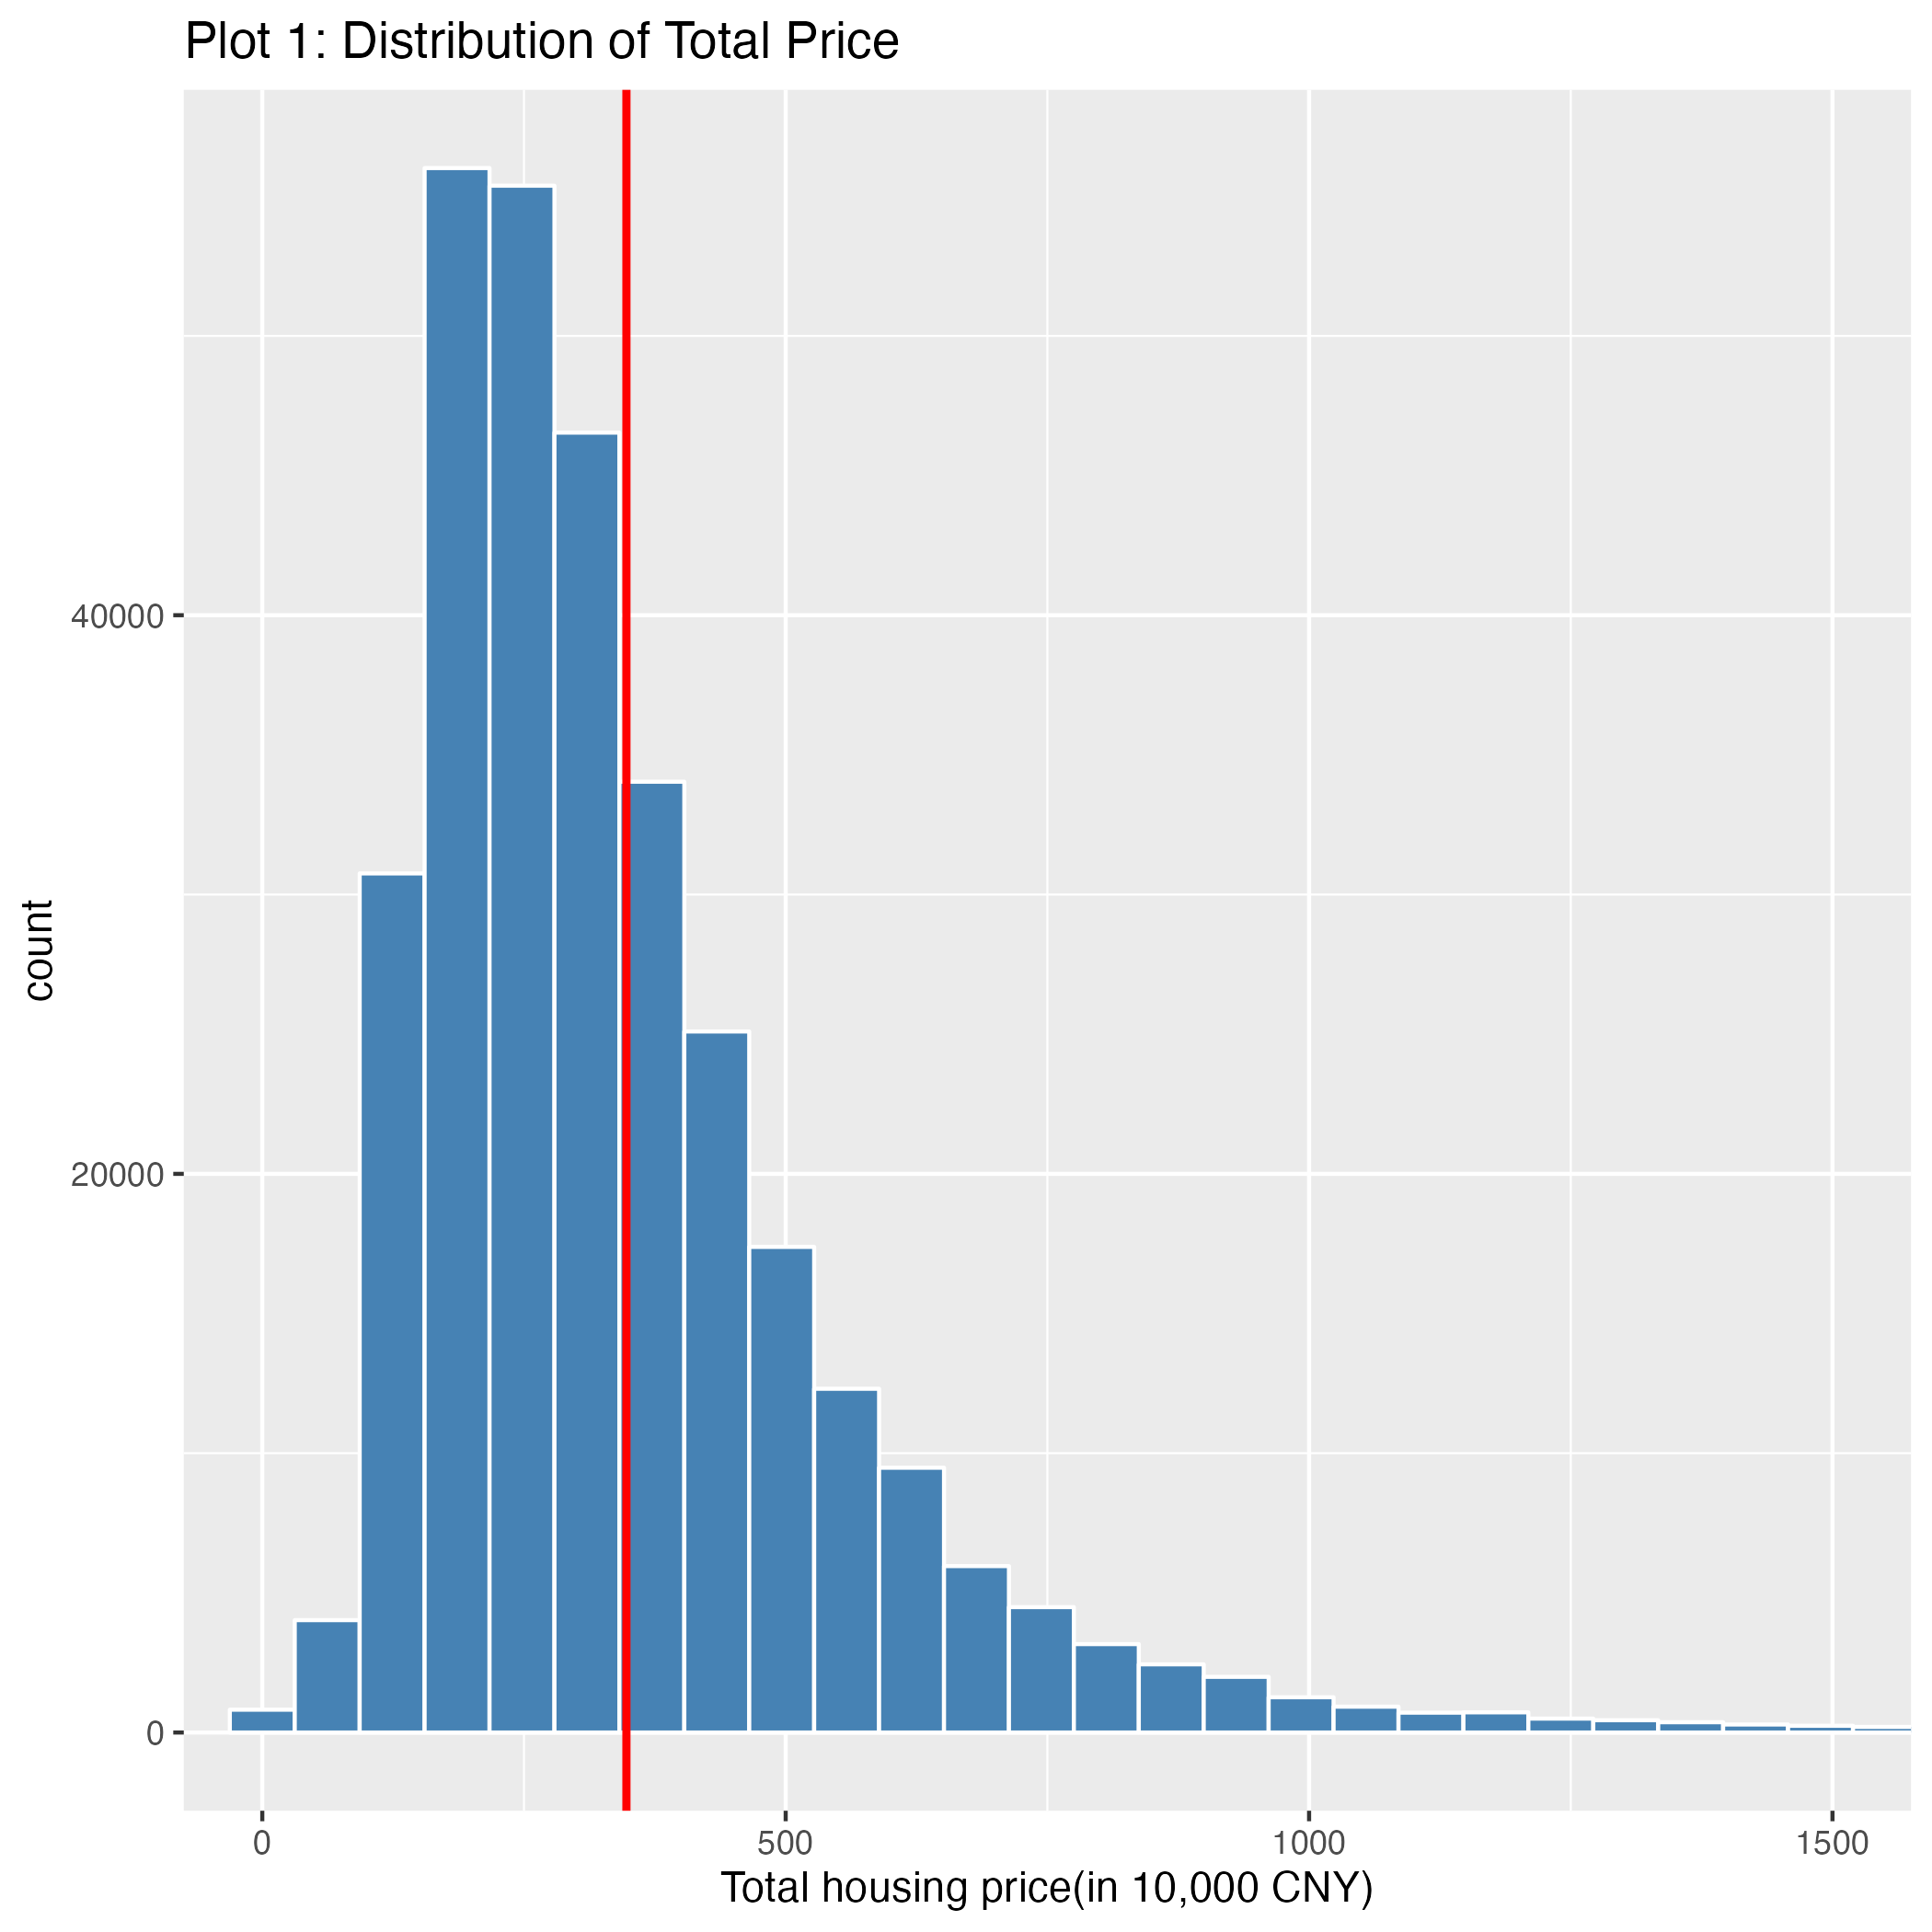
\includegraphics{../results/figure/plot_1_totalprice_distribution_plot.png}

}

\caption{\label{fig-totalprice-distribution}Housing Price of Beijing
from 2011 to 2017}

\end{figure}%

Upon curating a refined dataset, we embarked on exploratory data
analysis to unravel underlying patterns and associations.
Figure~\ref{fig-totalprice-distribution} showcased a histogram of total
prices, indicating a right-skewed distribution with a marked
concentration of lower-priced properties---a phenomenon underscored by
the mean or median price depicted through a central red line. This
visualization was pivotal in discerning the varied housing market range
within Beijing.

\begin{figure}

\centering{

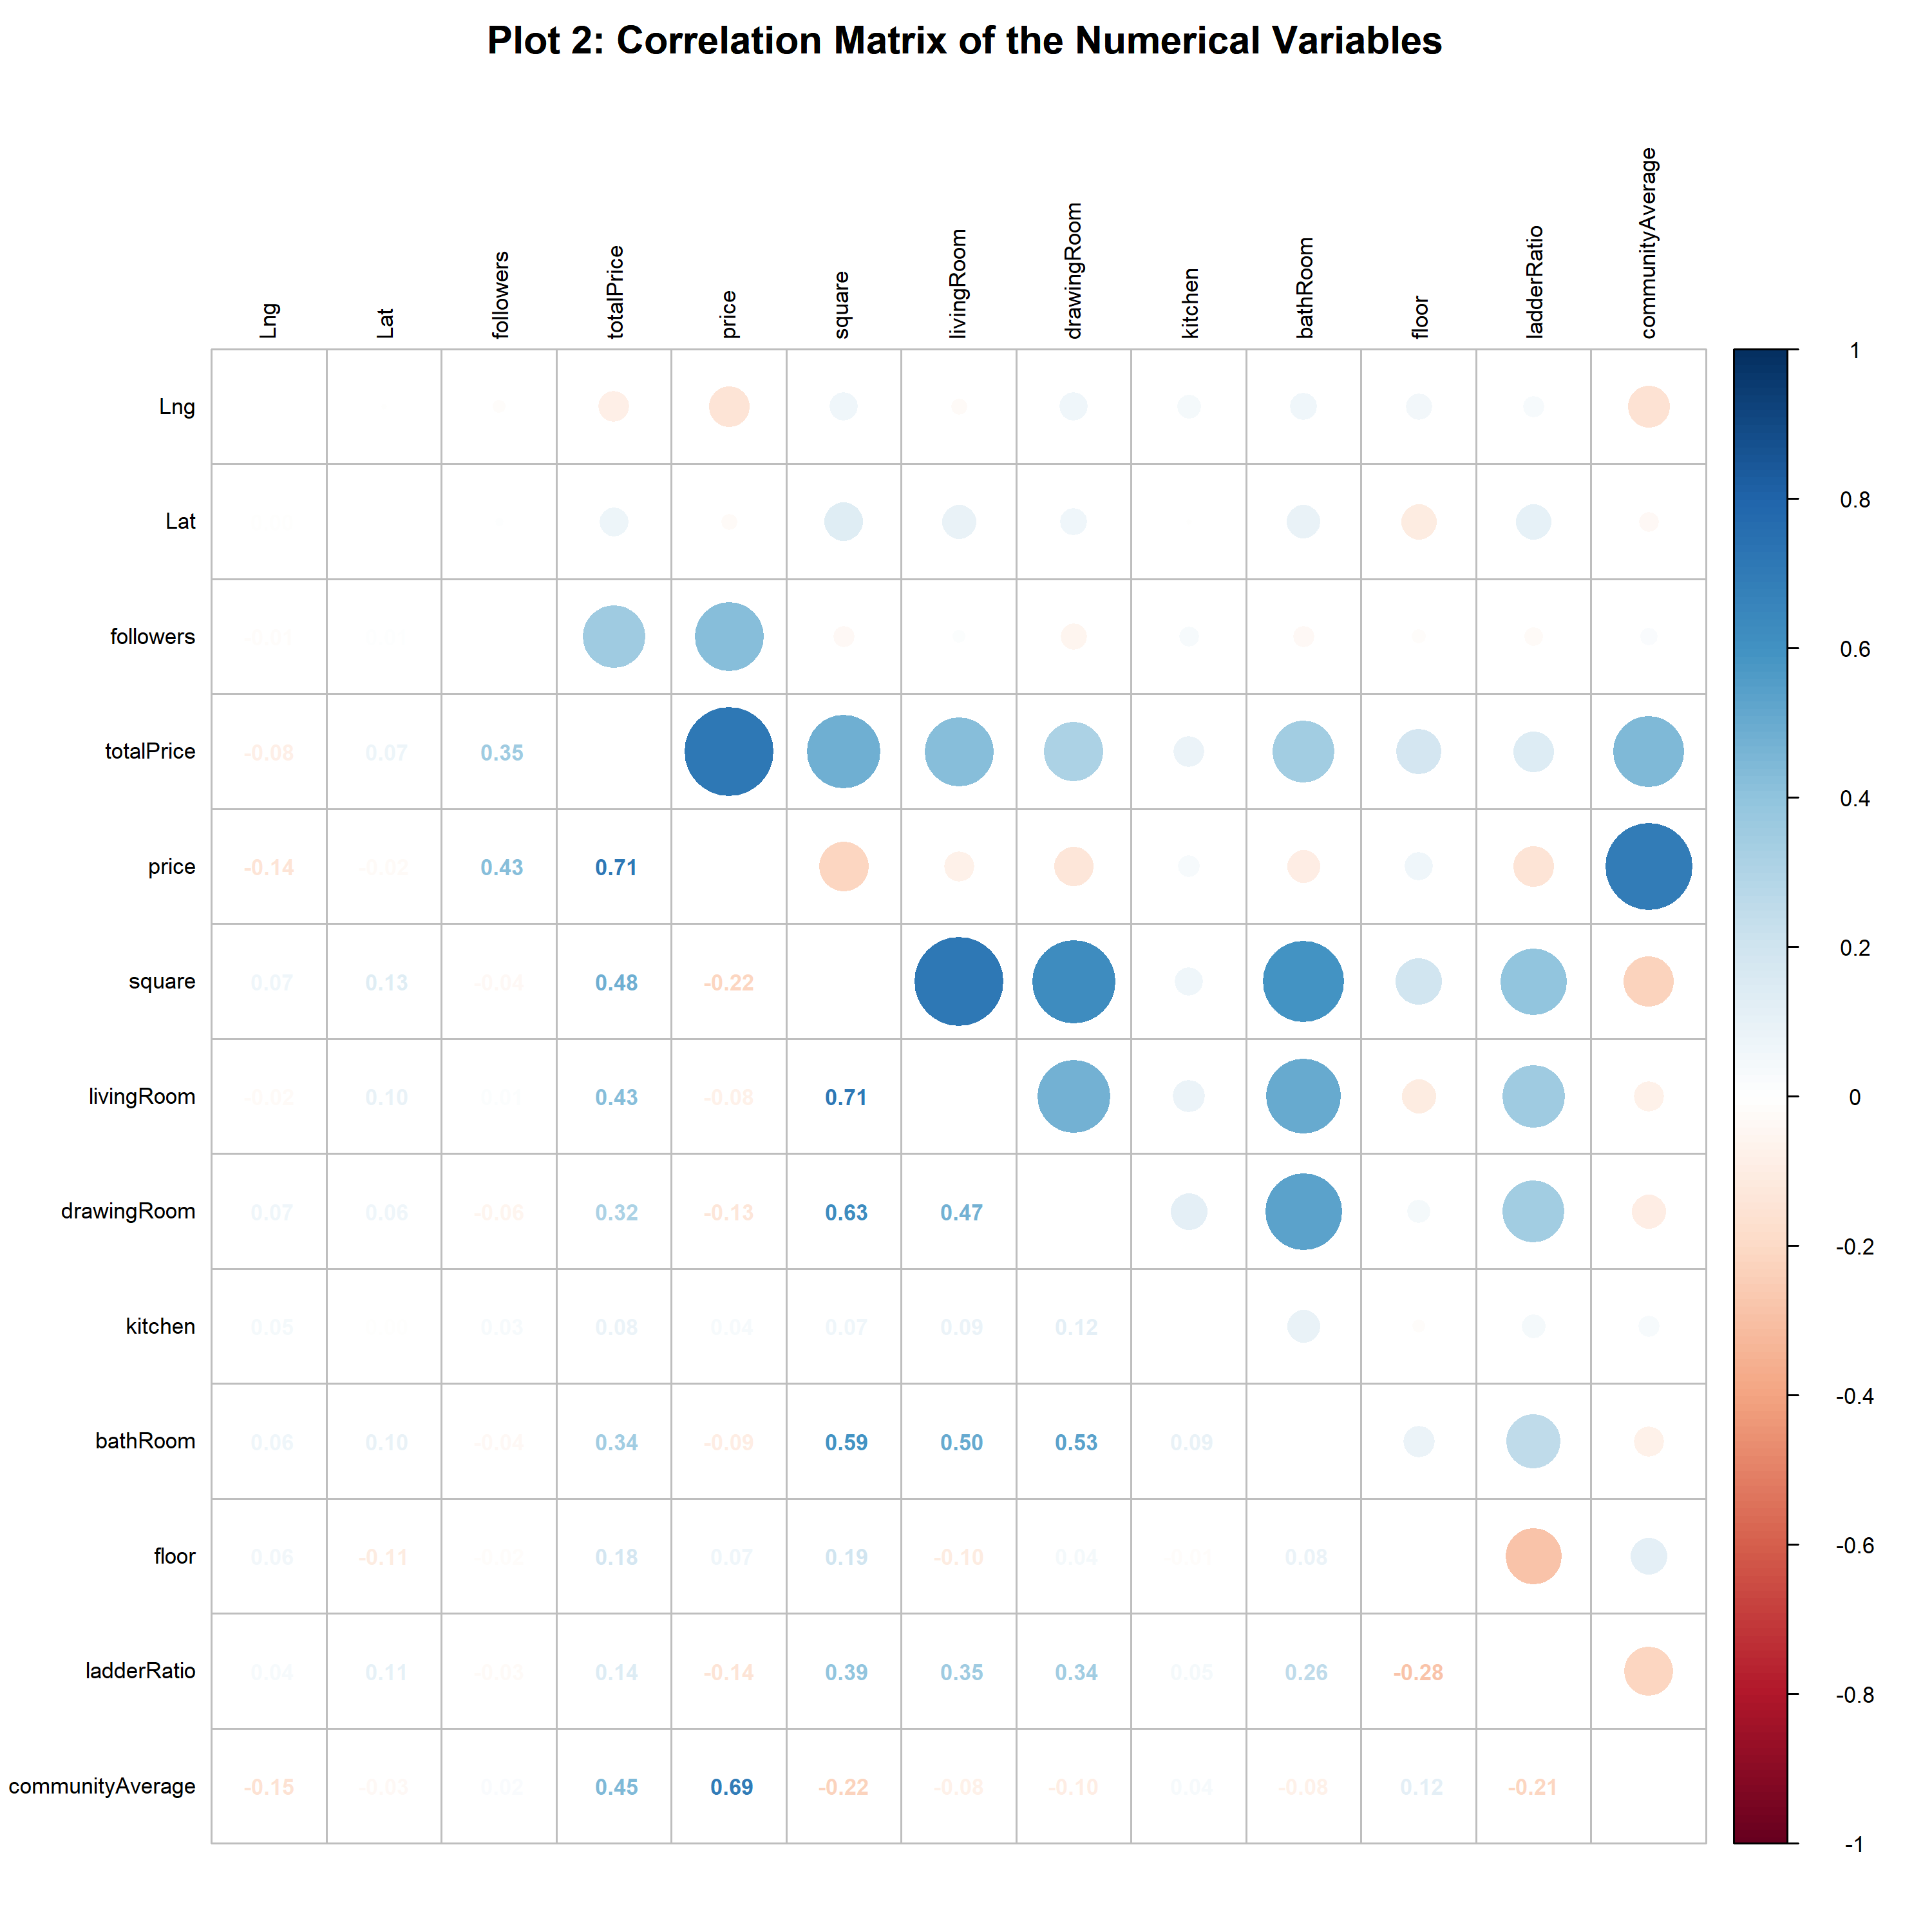
\includegraphics{../results/figure/plot_2_correlation_plot.png}

}

\caption{\label{fig-correlation}Correlation Between Variables}

\end{figure}%

In Figure~\ref{fig-correlation}, we computed and visualized a
correlation matrix to highlight potential linear relationships, with
circle sizes corresponding to the correlation strength. Notably, the
matrix revealed a prominent positive correlation between property size
and total price, suggesting a direct relationship between square footage
and market value.

\begin{figure}

\centering{

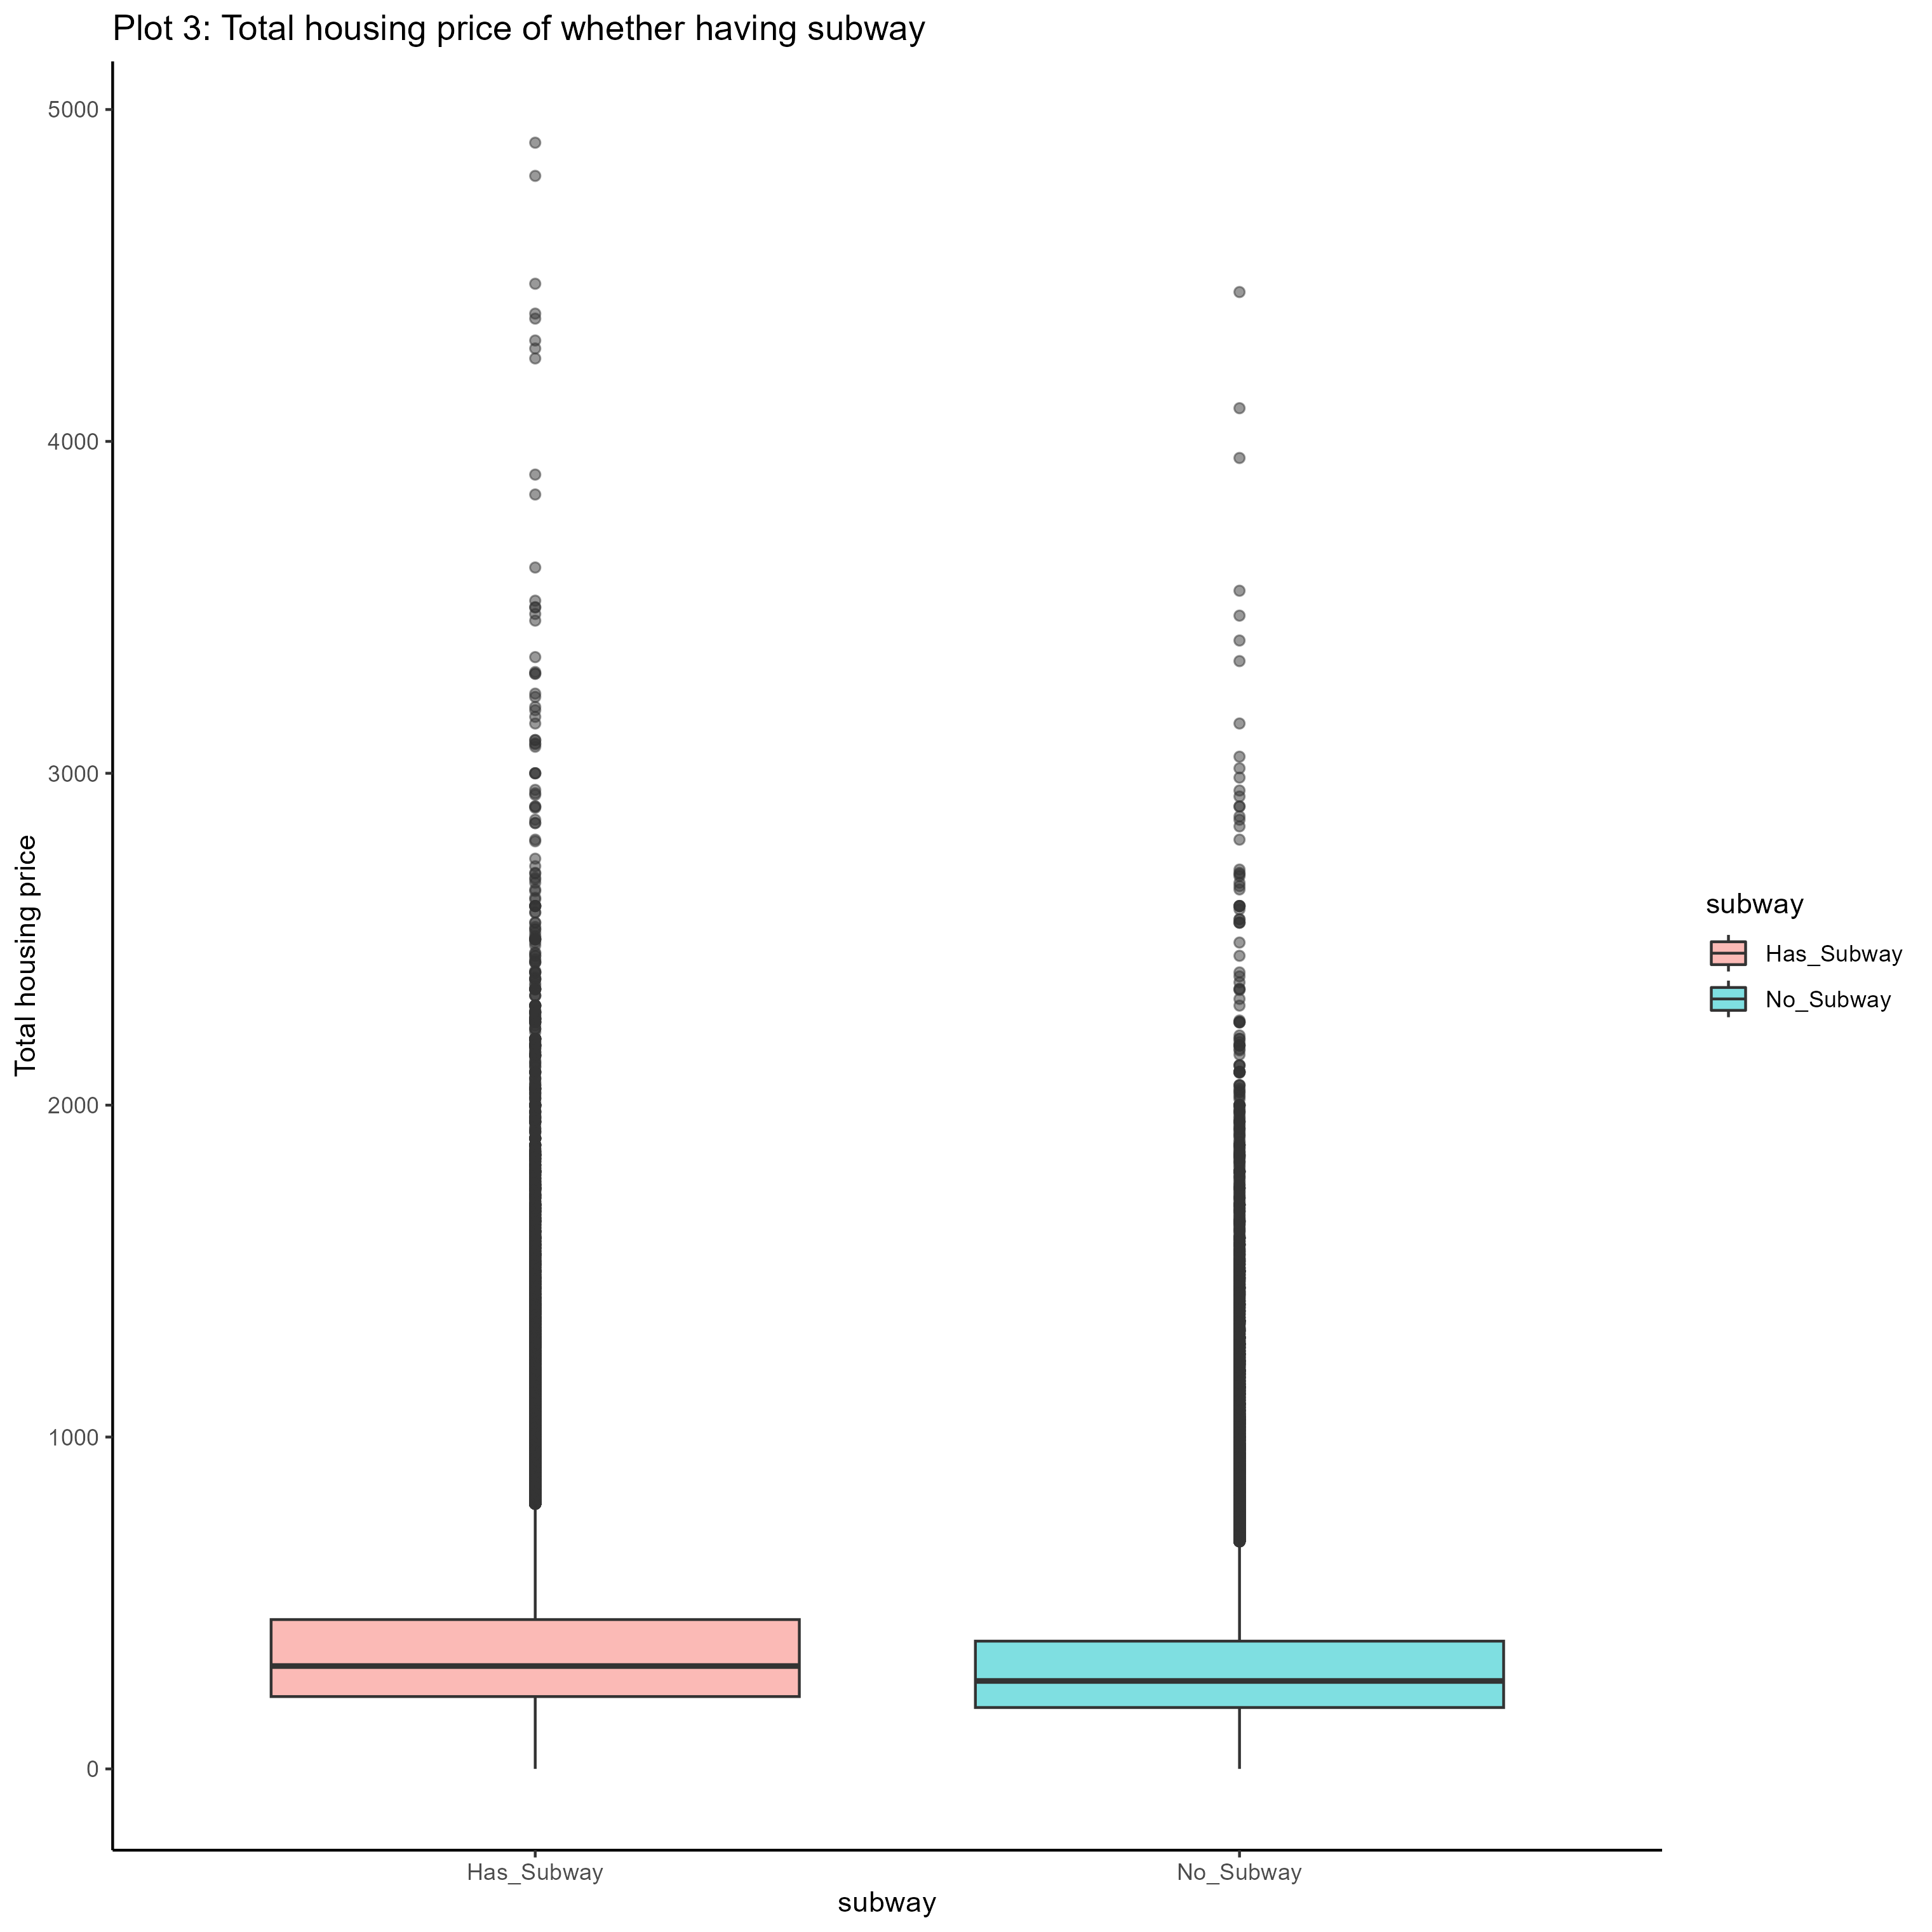
\includegraphics{../results/figure/plot_3_price_distribution_subway.png}

}

\caption{\label{fig-subway-distribution}Total Housing Price of Whether
Having Subway}

\end{figure}%

\begin{figure}

\centering{

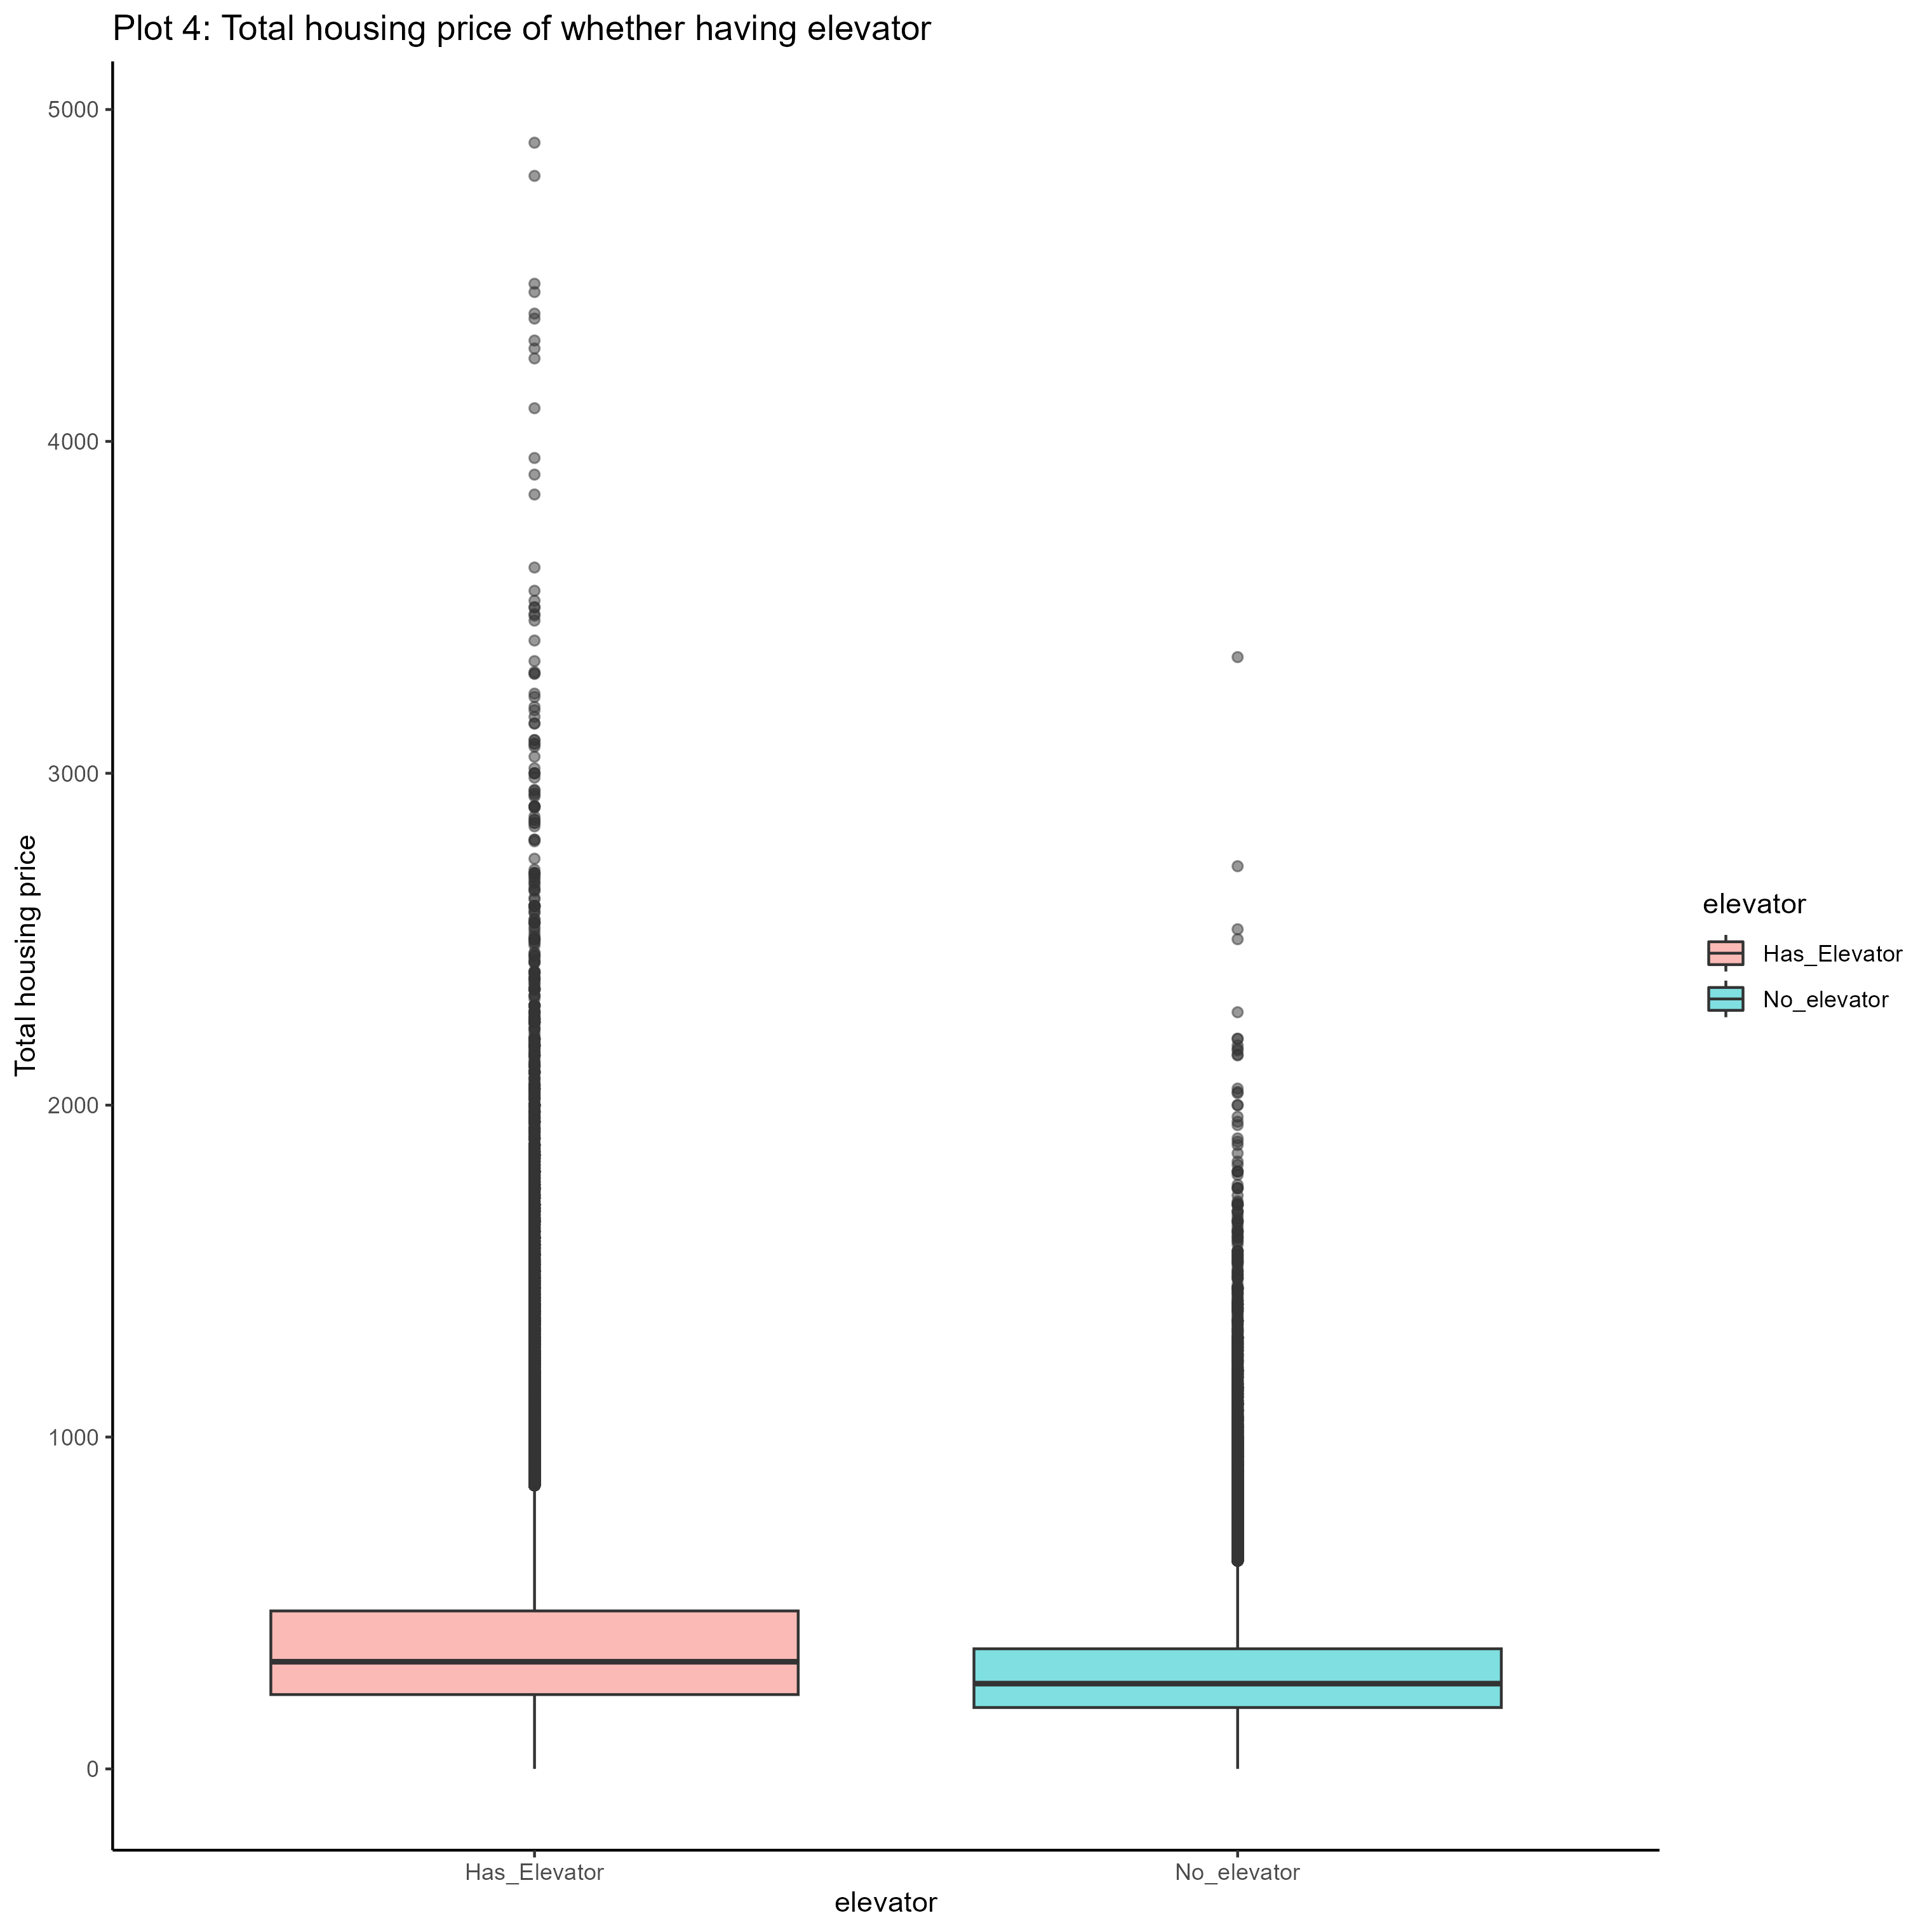
\includegraphics{../results/figure/plot_4_price_distribution_elevator.png}

}

\caption{\label{fig-elevator-distribution}Total housing Price of Whether
Having Elevator}

\end{figure}%

The value of property features was illustrated in
Figure~\ref{fig-subway-distribution} and
Figure~\ref{fig-elevator-distribution} through box plots comparing total
prices based on the presence of subways and elevators. The premium for
these features was clearly visible, reflecting the higher prices
consumers are willing to pay for added convenience.

\begin{figure}

\centering{

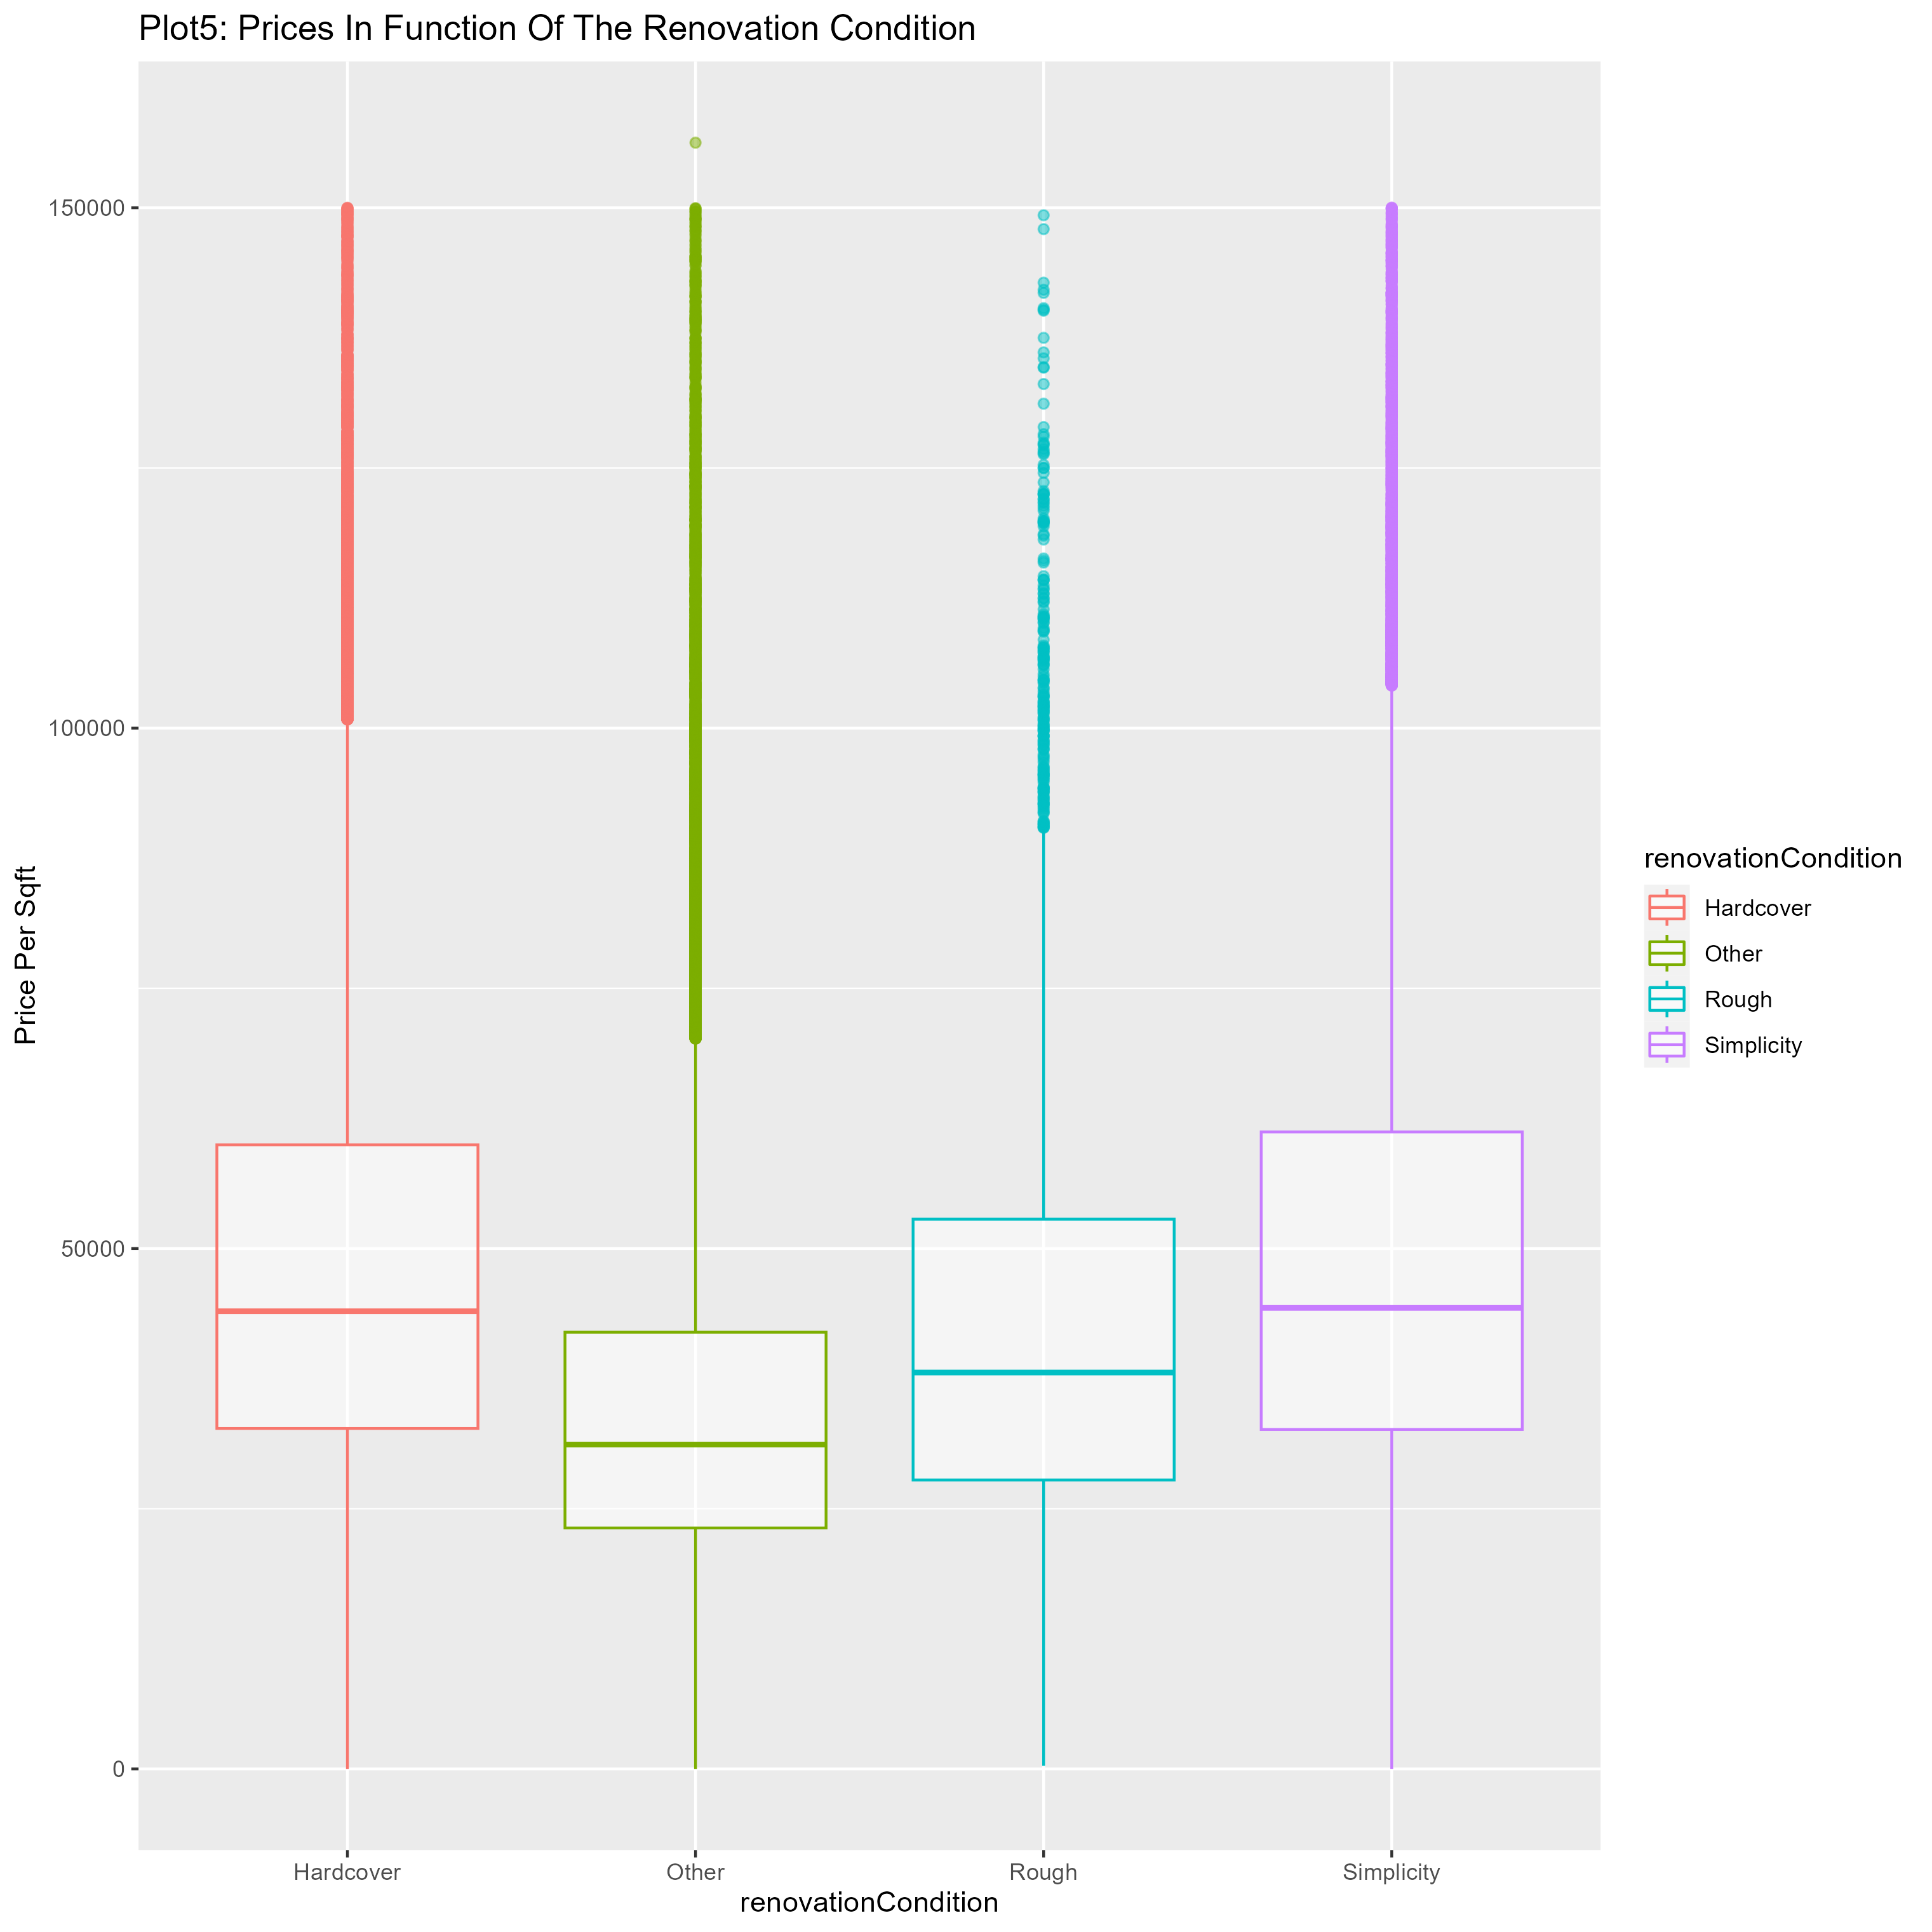
\includegraphics{../results/figure/plot_5_renovation_condition.png}

}

\caption{\label{fig-renovation-condition}Prices in Function of The
Renovation Condition}

\end{figure}%

Figure~\ref{fig-renovation-condition} delved into the impact of
renovation conditions on property values. Through the variance
illustrated in the box plots for each condition category, we observed a
correlation between renovation quality and pricing, indicating that
buyers are inclined to invest more in well-maintained properties.

\begin{figure}

\centering{

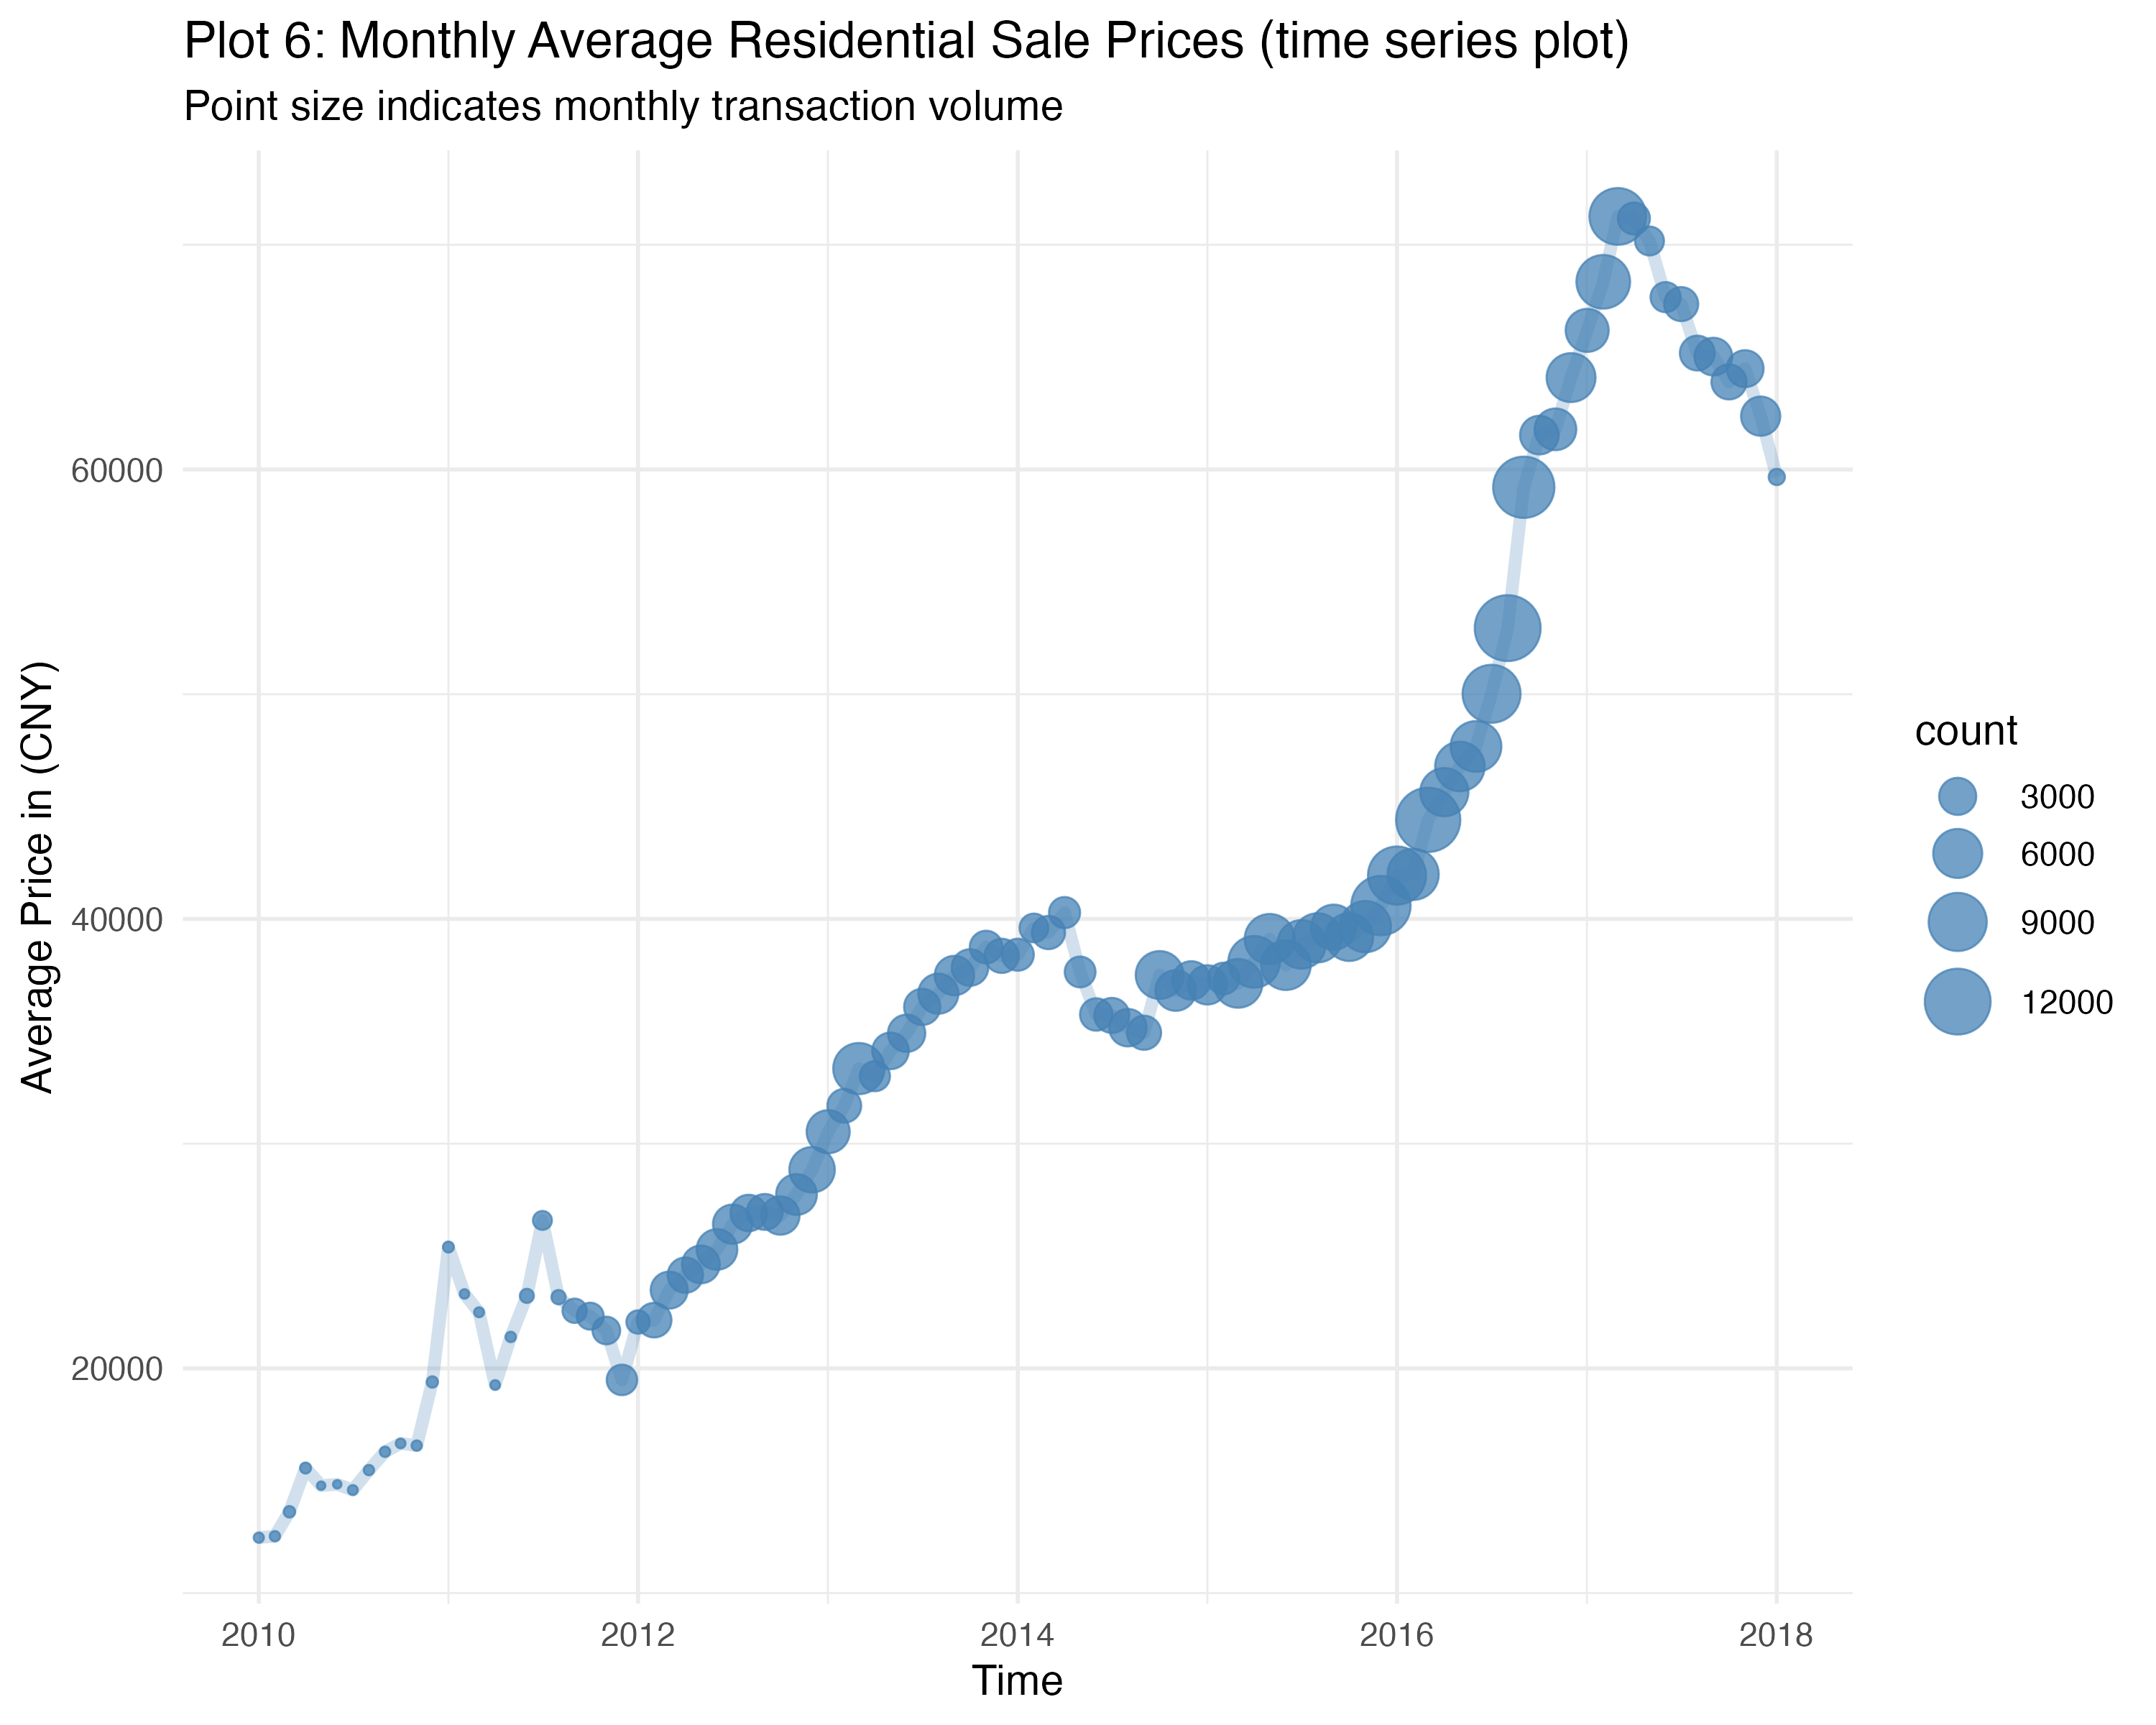
\includegraphics{../results/figure/plot_6_monthly_price_overview.png}

}

\caption{\label{fig-monthly-price}Monthly Average Residential Sale
Price}

\end{figure}%

The market's temporal dynamics were captured in
Figure~\ref{fig-monthly-price}, a time series plot that traced the
trajectory of average monthly residential sale prices, with the volume
of transactions visually represented by the size of the points. This
plot served as an indicator of market trends and economic factors
affecting housing prices over time.

\begin{figure}

\centering{

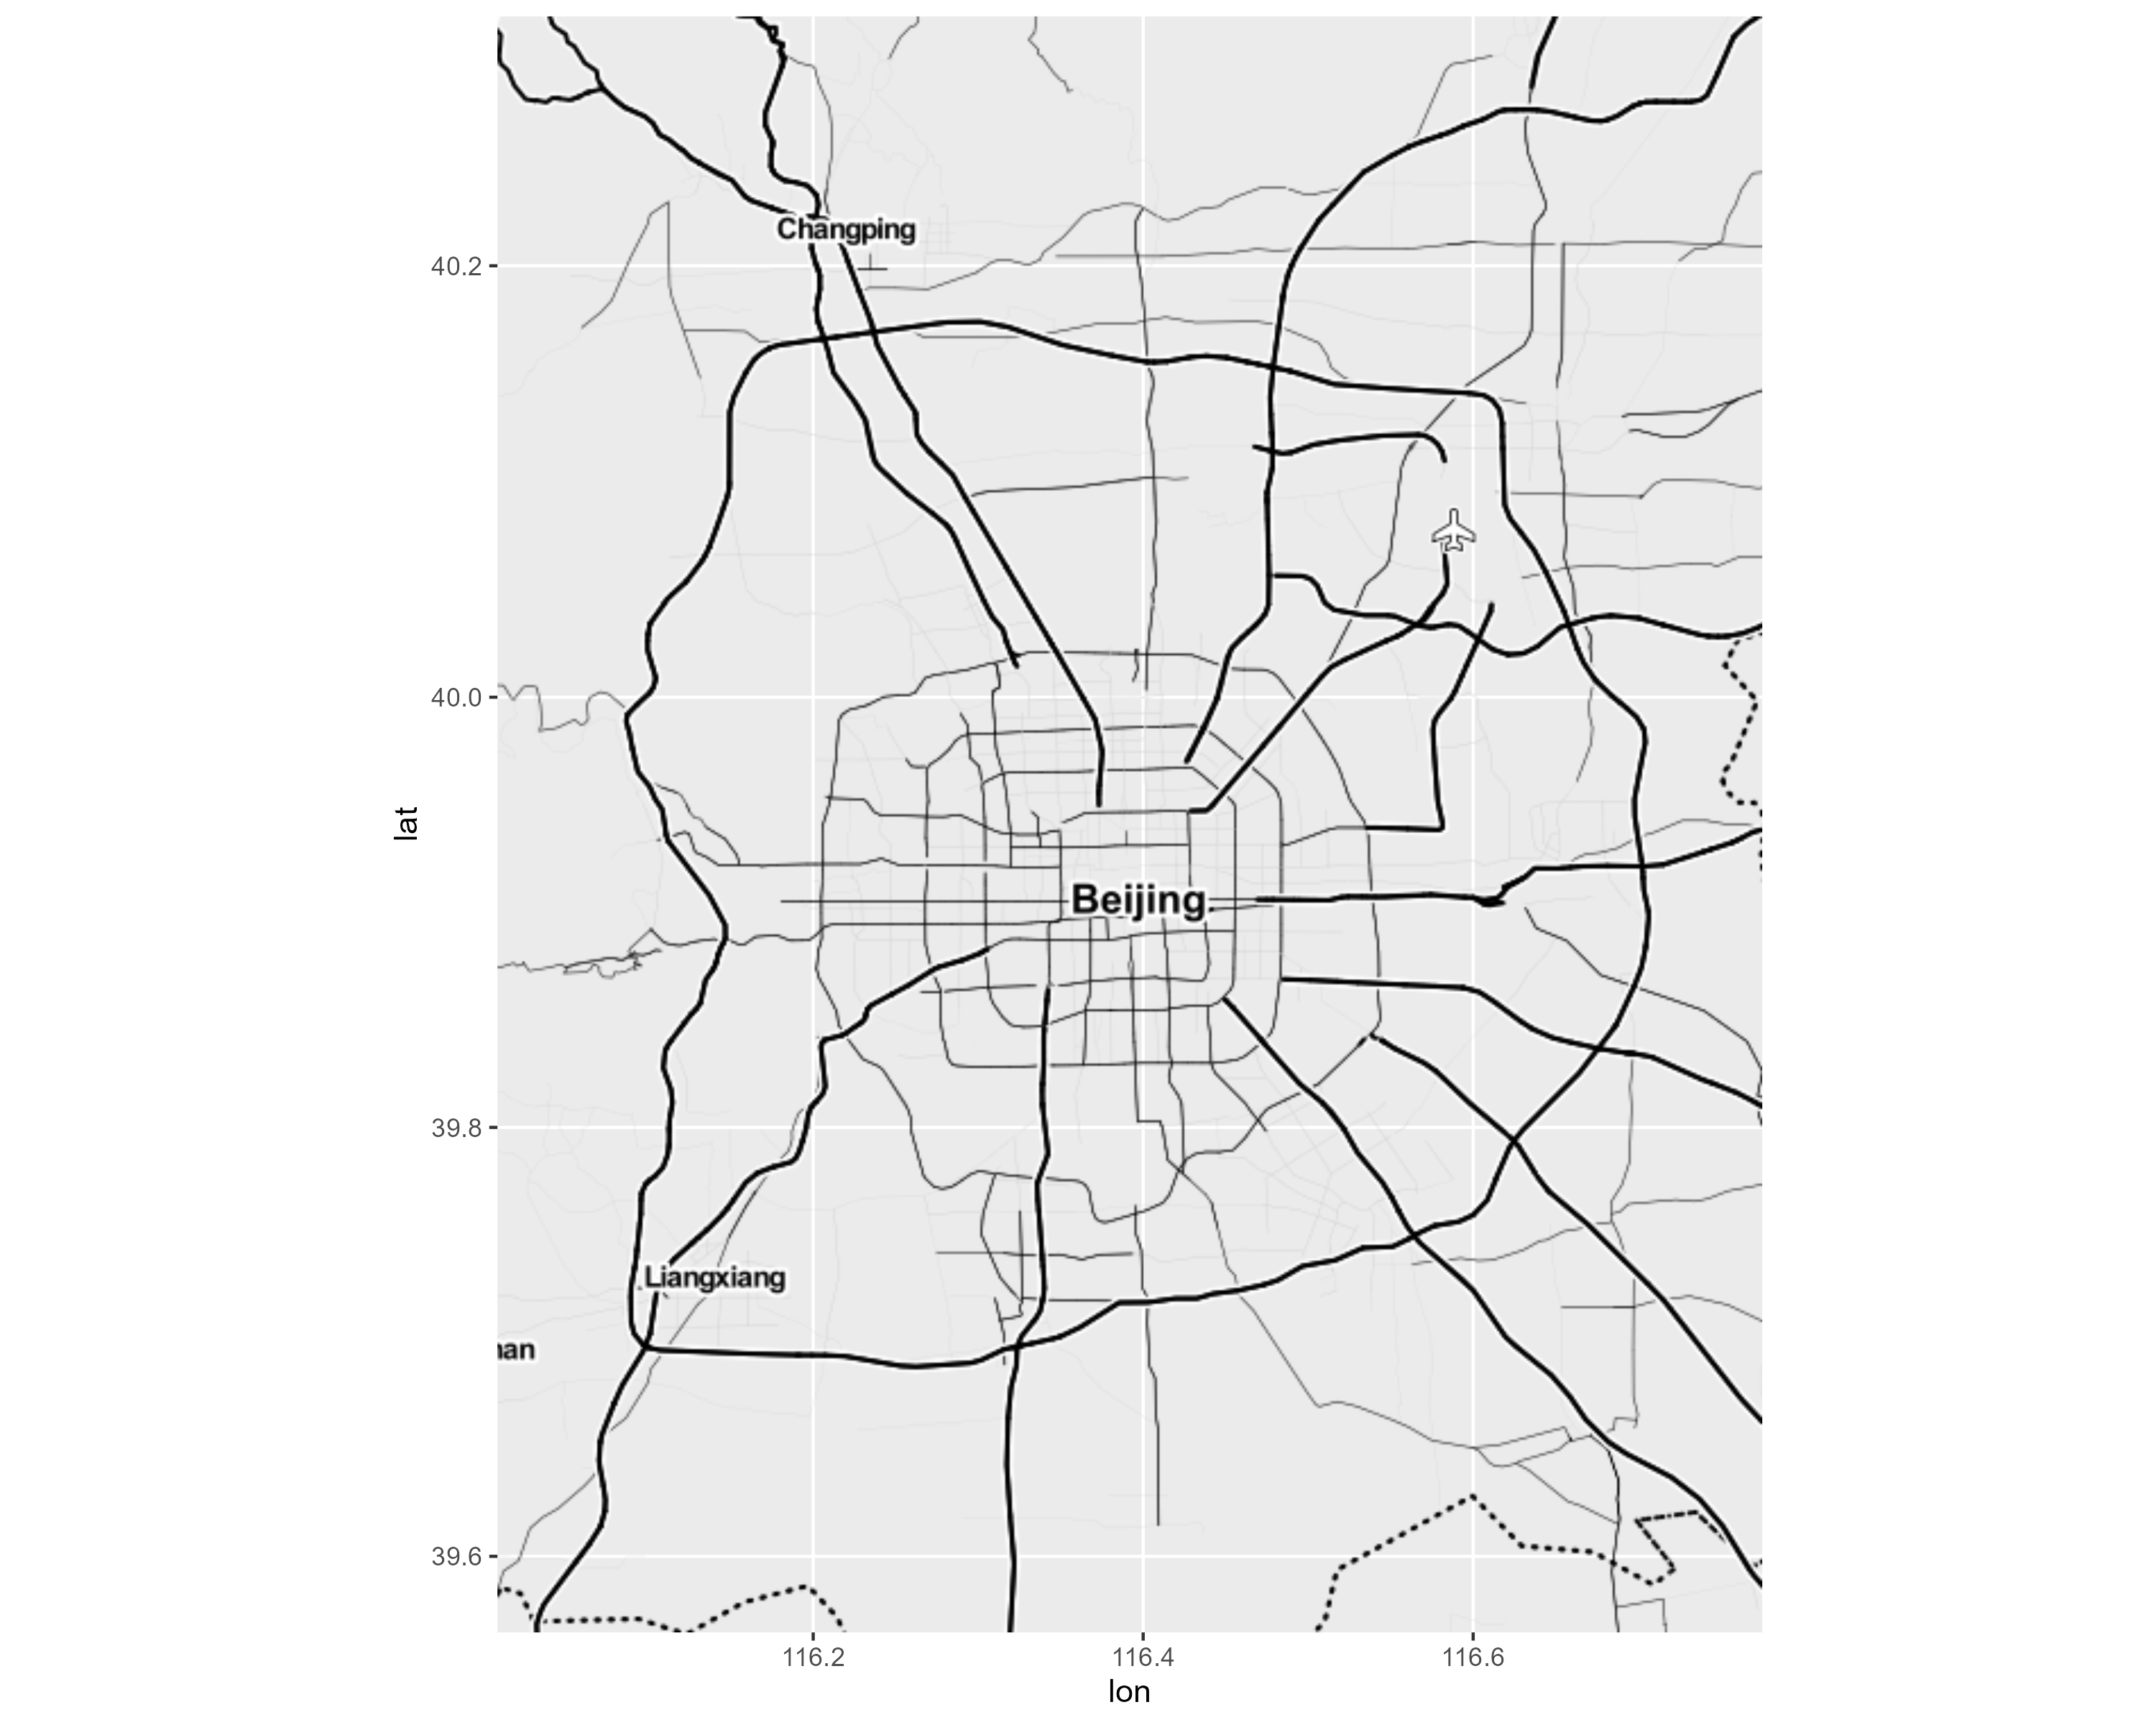
\includegraphics{../results/figure/plot_7_beijing_map.png}

}

\caption{\label{fig-beijing-map}Beijing Map}

\end{figure}%

\begin{figure}

\centering{

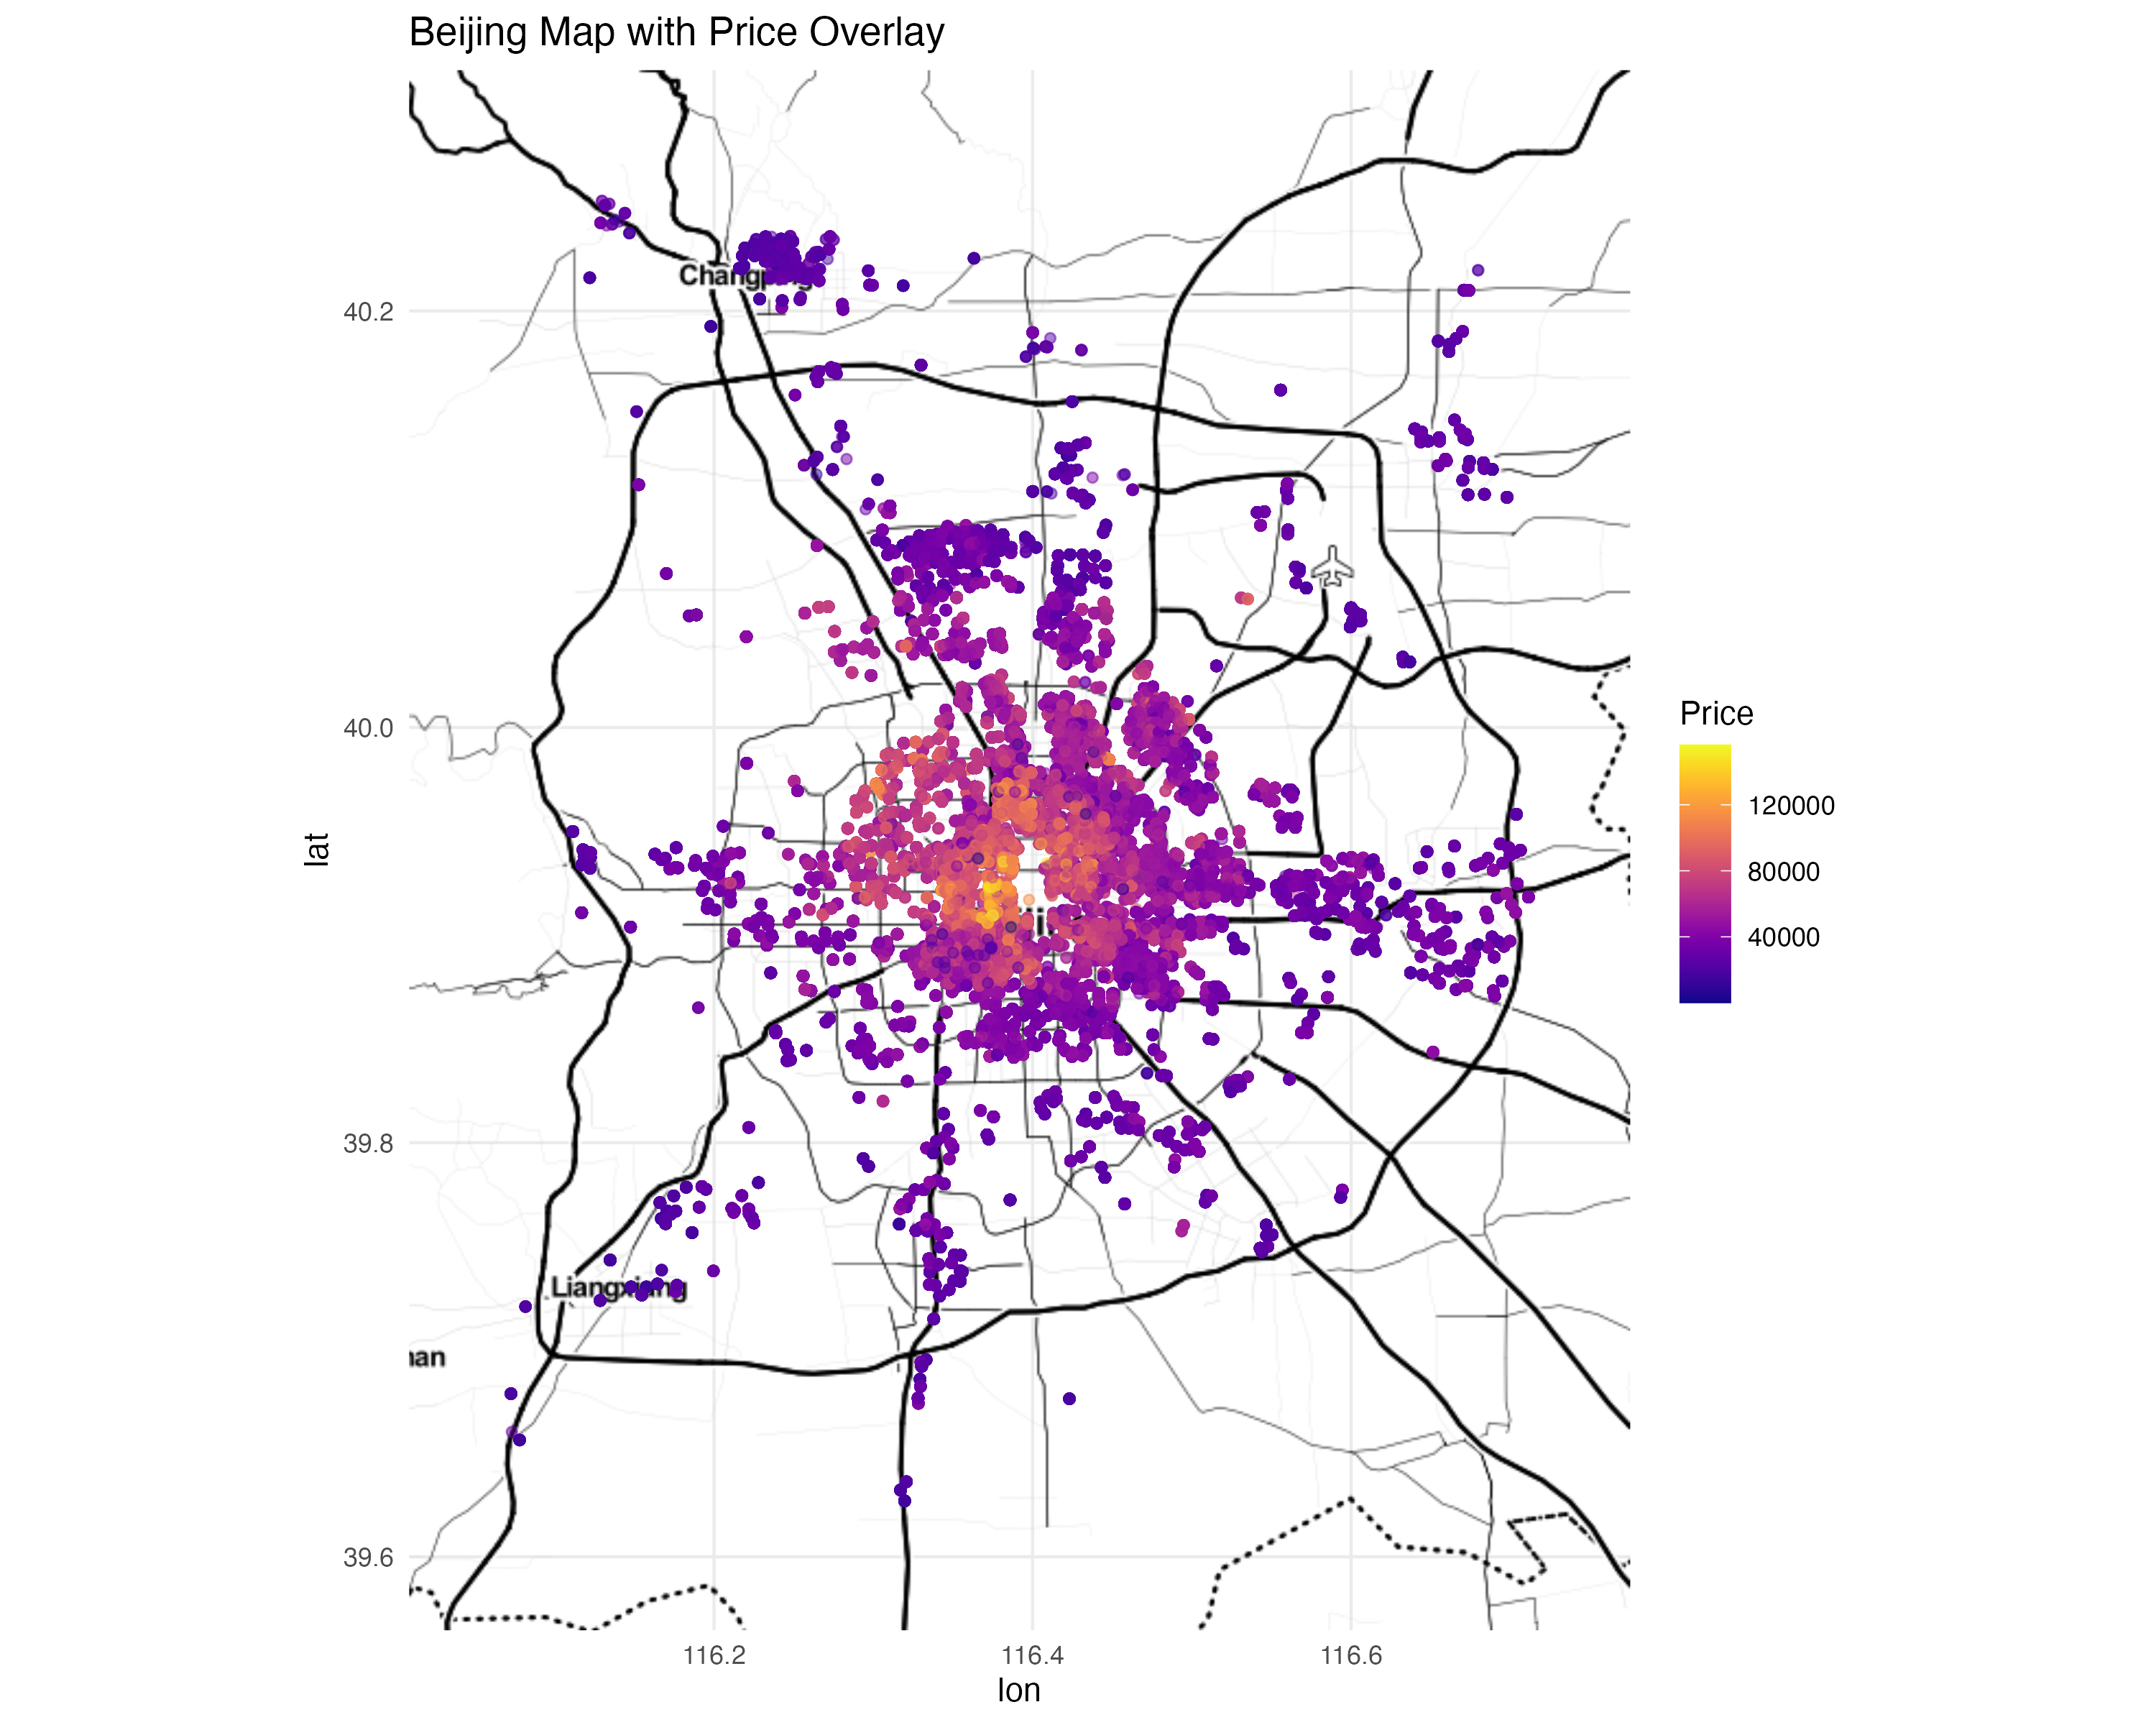
\includegraphics{../results/figure/plot_8_beijing_map_with_price_overlay.png}

}

\caption{\label{fig-beijing-map-with-price}Map with Housing Price}

\end{figure}%

Geospatial distribution and its influence on property values were
elucidated through Figure~\ref{fig-beijing-map} and
Figure~\ref{fig-beijing-map-with-price}. A base map of Beijing provided
the context for a subsequent overlay of price data, revealing distinct
high and low-value areas across the cityscape.

\begin{figure}

\centering{

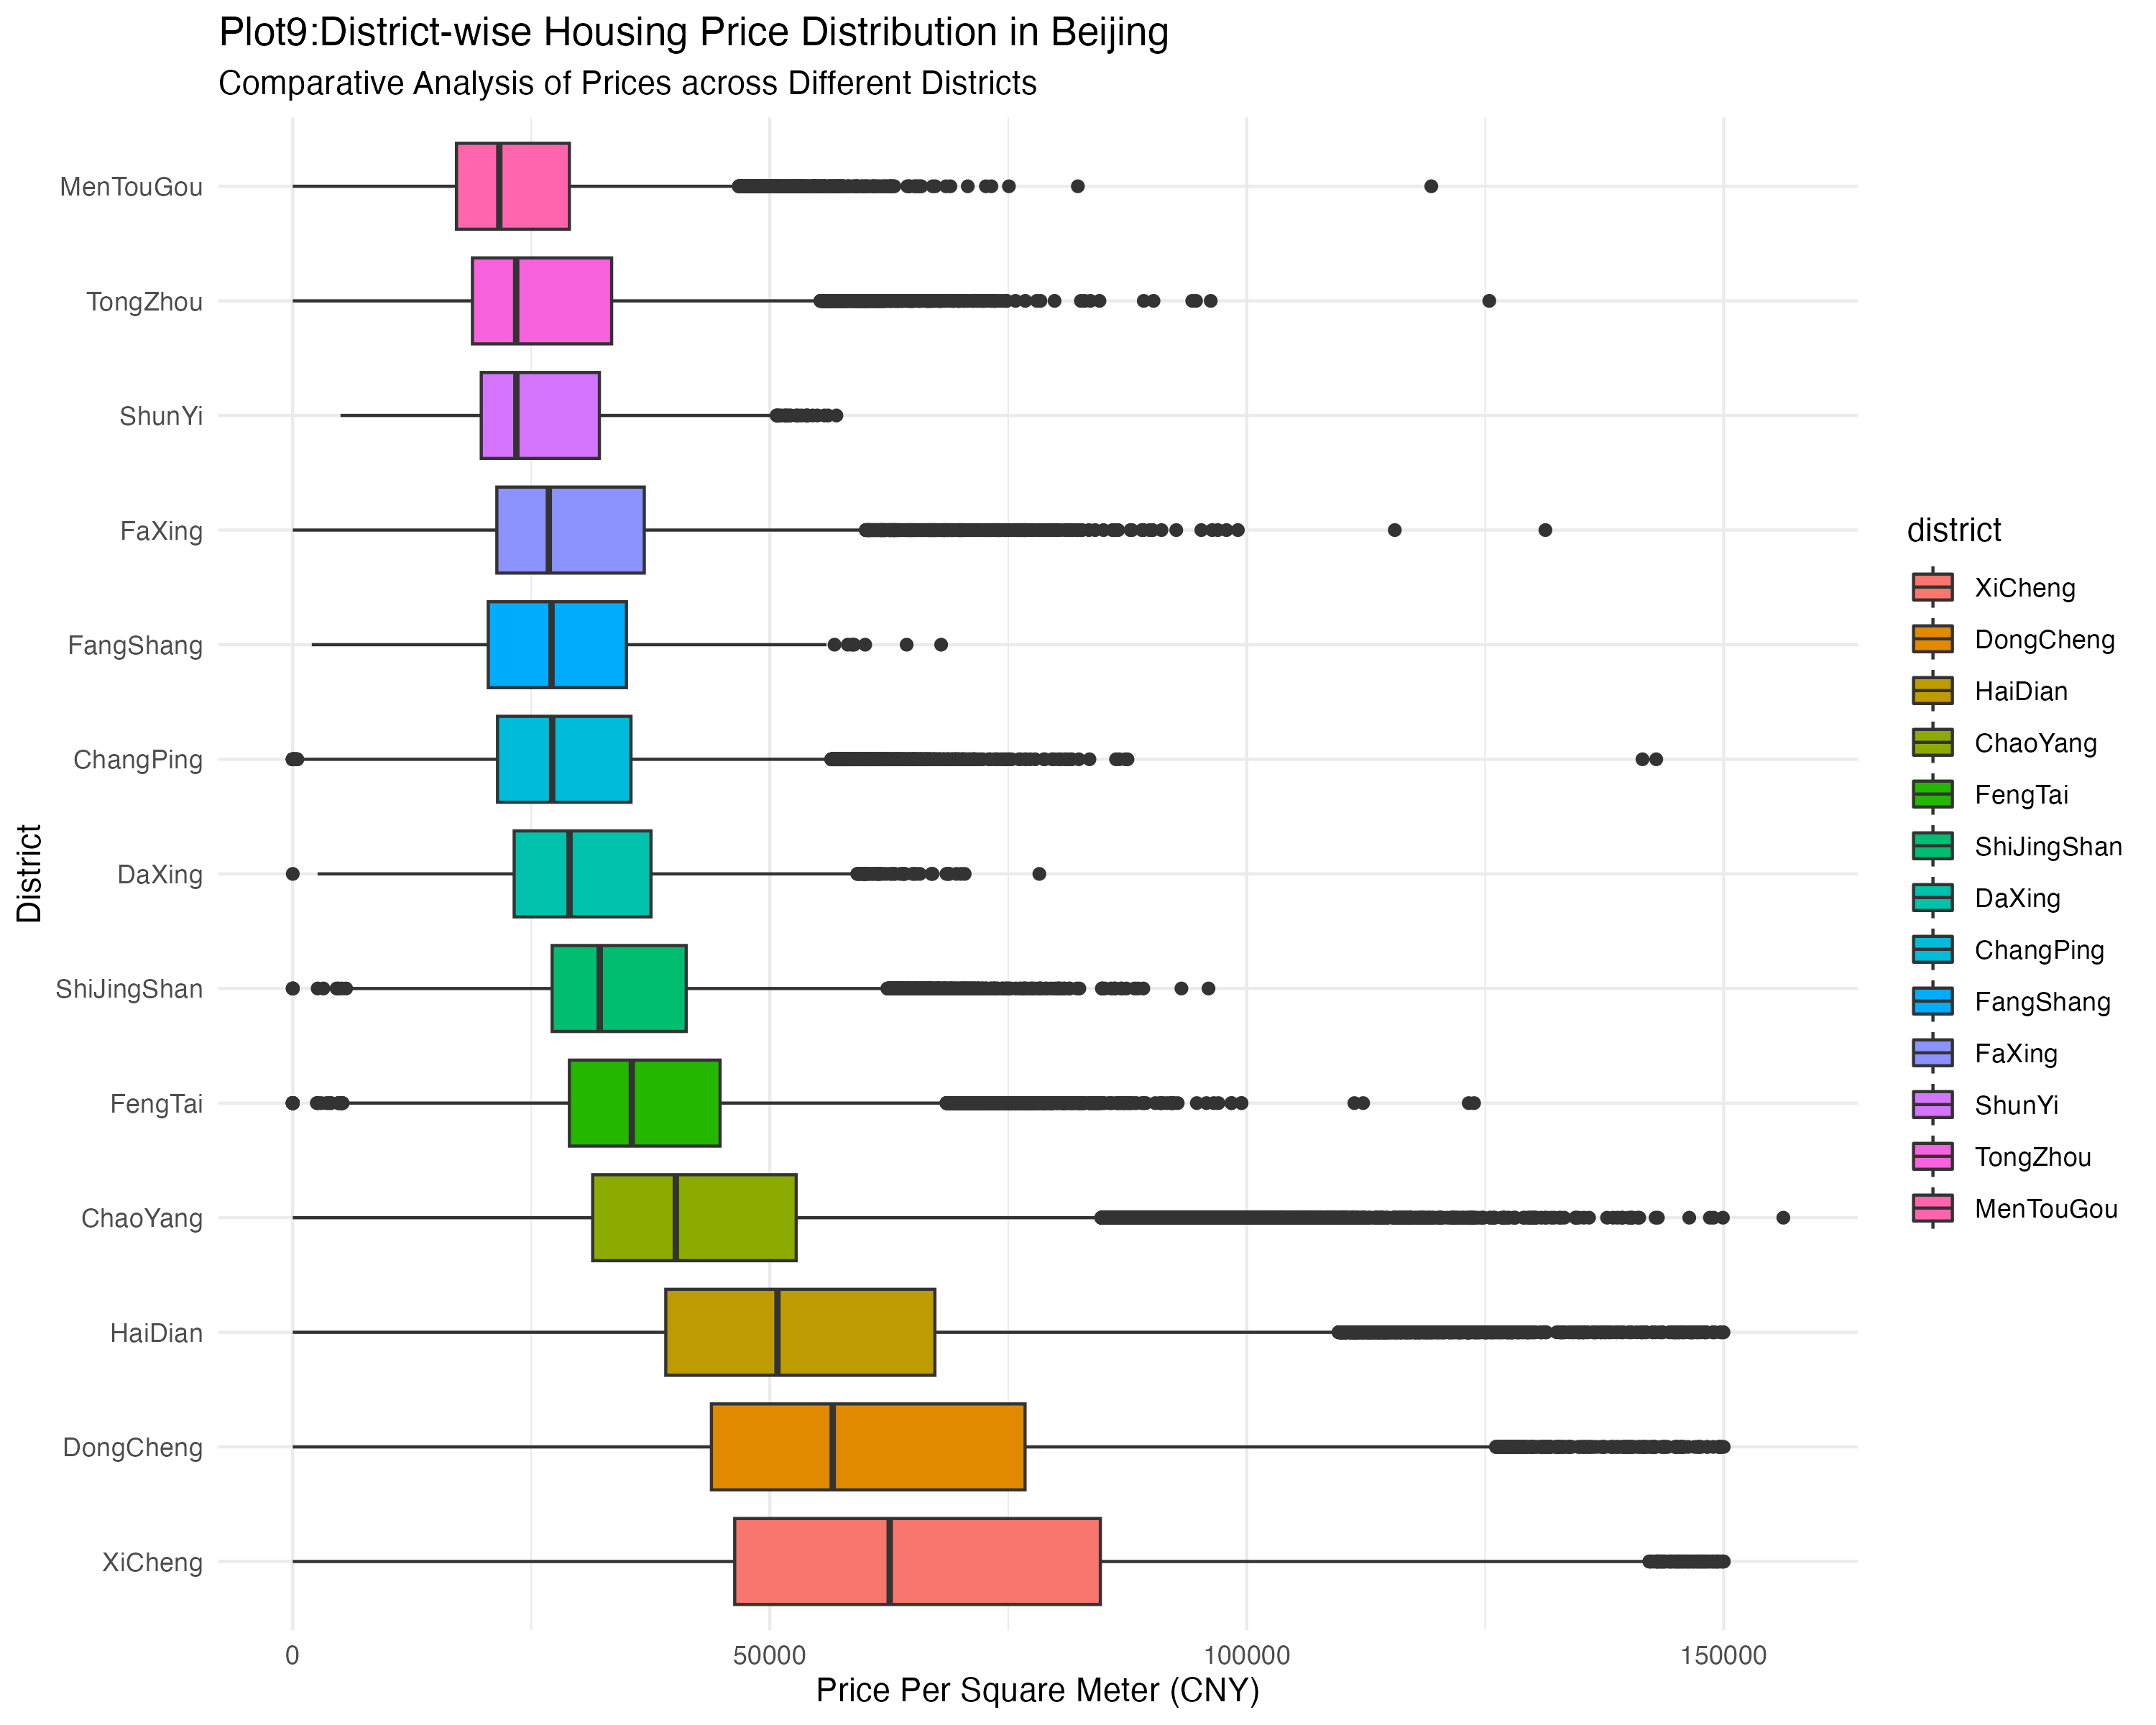
\includegraphics{../results/figure/plot_9_boxplot_price_district.png}

}

\caption{\label{fig-district-wise-housing-price}District-wise Housing
Price Distribution}

\end{figure}%

Figure~\ref{fig-district-wise-housing-price} presented a detailed
district-wise analysis, comparing housing prices across Beijing's
various districts through box plots. This granular view highlighted the
real estate disparities influenced by district-specific characteristics.

\begin{figure}

\centering{

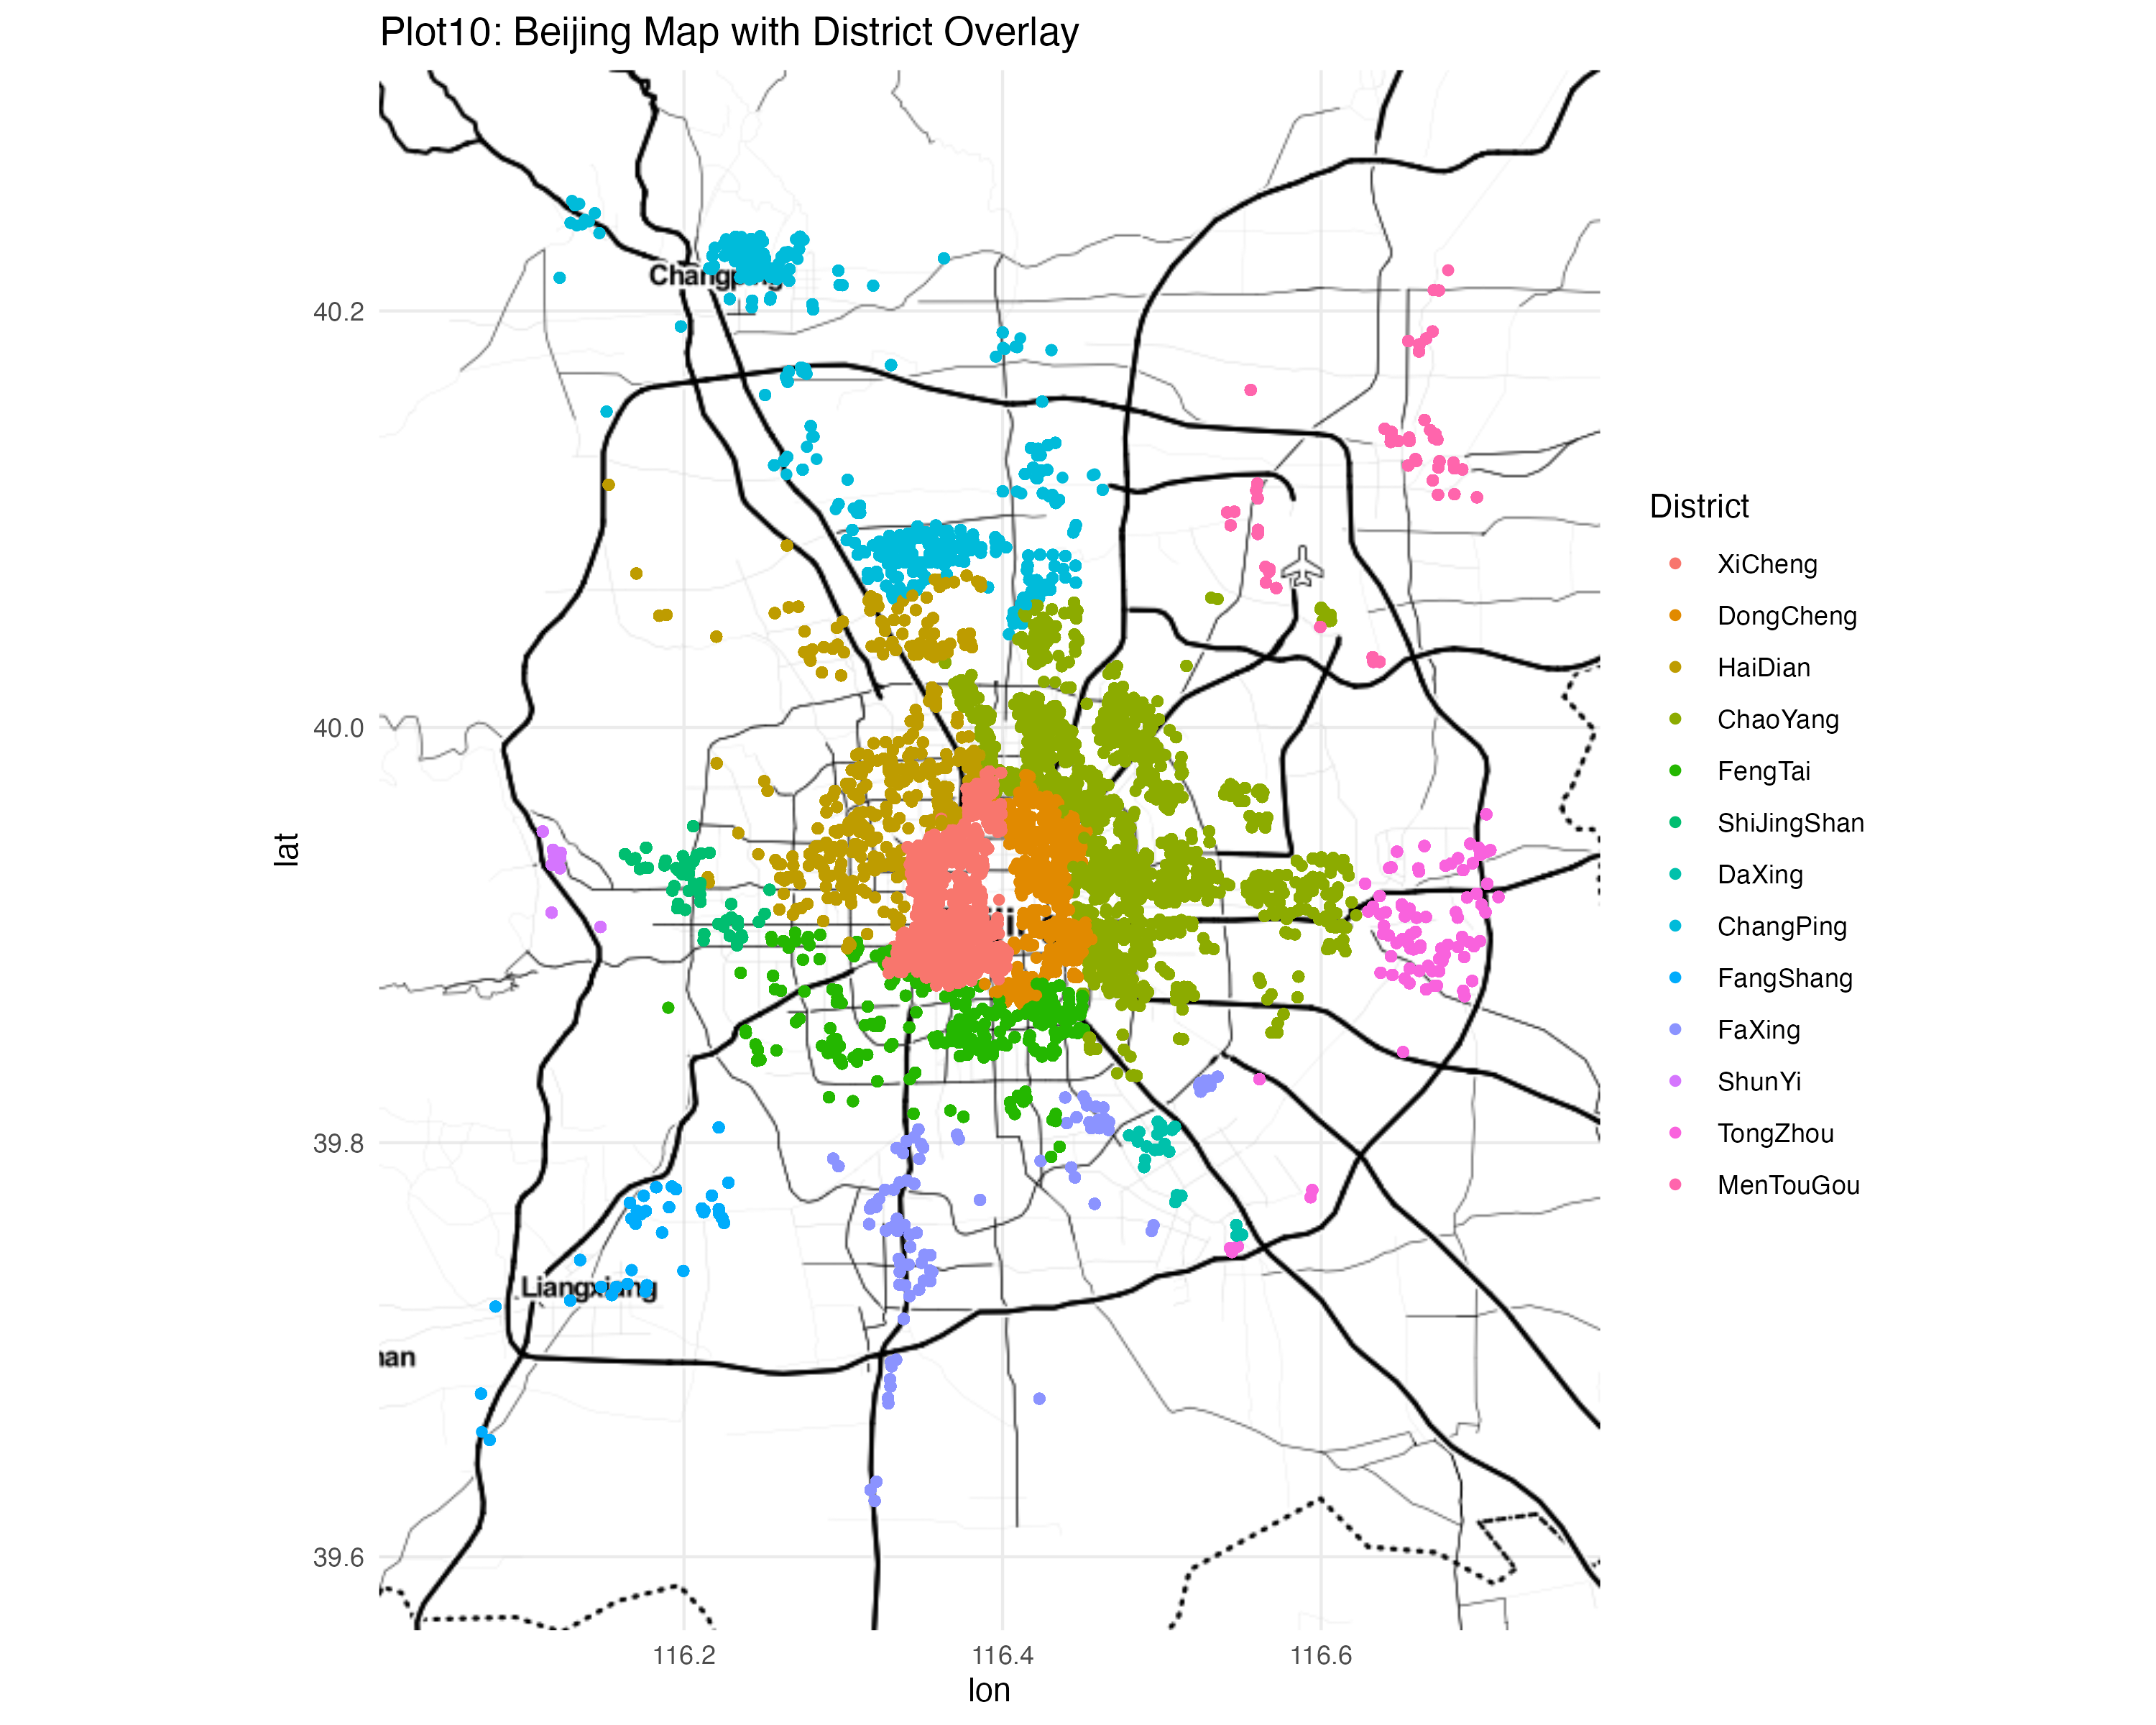
\includegraphics{../results/figure/plot_10_beijing_map_with_district_overlay.png}

}

\caption{\label{fig-beijing-map-with-district}Beijing Map with District
Overlay}

\end{figure}%

Finally, Figure~\ref{fig-beijing-map-with-district} combined geographic
and price data by color-coding each district on a map of Beijing,
offering an at-a-glance comparison of real estate valuation across
different urban areas.

Our linear regression model, developed after the exploratory analysis,
utilized these processed and visualized data to predict total property
prices. The model's efficacy was visually assessed by overlaying actual
versus predicted prices on a scatter plot, which served as a testament
to the model's predictive capabilities. The careful curation and
analysis of the dataset provided insights into the market drivers for
housing prices in Beijing, which could aid stakeholders in making
data-driven decisions.

\subsection{Result}\label{result}

\begin{table}

\caption{\label{tbl-model}}

\centering{

\captionsetup{labelsep=none}

\begin{verbatim}

Call:
lm(formula = totalPrice ~ . - constructionTime - buildingType, 
    data = beijing_house_price)

Residuals:
     Min       1Q   Median       3Q      Max 
-1596.36   -25.86     1.62    29.21  2522.00 

Coefficients:
                                      Estimate Std. Error t value Pr(>|t|)    
(Intercept)                          7.094e+03  3.970e+02  17.868  < 2e-16 ***
Lng                                 -7.155e+01  2.970e+00 -24.090  < 2e-16 ***
Lat                                  1.240e+01  3.415e+00   3.630 0.000283 ***
tradeTime                            1.943e-02  4.687e-04  41.454  < 2e-16 ***
followers                            1.010e-02  4.456e-03   2.267 0.023404 *  
price                                7.044e-03  1.378e-05 511.325  < 2e-16 ***
square                               4.493e+00  7.836e-03 573.444  < 2e-16 ***
livingRoom                          -3.137e+00  2.777e-01 -11.294  < 2e-16 ***
drawingRoom                         -8.287e+00  3.450e-01 -24.020  < 2e-16 ***
kitchen                              1.427e+01  1.408e+00  10.134  < 2e-16 ***
bathRoom                            -1.207e+01  4.808e-01 -25.092  < 2e-16 ***
floor                               -2.213e-01  2.913e-02  -7.600 2.97e-14 ***
renovationConditionOther             8.163e-01  4.375e-01   1.866 0.062085 .  
renovationConditionRough            -1.522e+01  1.095e+00 -13.900  < 2e-16 ***
renovationConditionSimplicity       -9.305e+00  3.685e-01 -25.254  < 2e-16 ***
buildingStructureBrick/Wood         -2.206e+02  8.732e+00 -25.261  < 2e-16 ***
buildingStructureMixed               5.619e+00  6.951e-01   8.085 6.26e-16 ***
buildingStructureSteel               6.469e+00  6.202e+00   1.043 0.296900    
buildingStructureSteel/Concrete      2.215e+01  8.336e-01  26.574  < 2e-16 ***
buildingStructureUnavailable        -1.768e+00  1.150e+01  -0.154 0.877831    
ladderRatio                         -2.565e-06  5.440e-06  -0.472 0.637225    
elevatorNo_elevator                  4.545e+00  5.982e-01   7.599 3.00e-14 ***
fiveYearsPropertyOwnership > 5years  4.461e-01  2.999e-01   1.488 0.136828    
subwayNo_Subway                      2.131e+00  3.076e-01   6.927 4.31e-12 ***
districtChaoYang                     4.417e+01  7.965e-01  55.447  < 2e-16 ***
districtDaXing                       3.773e+01  1.912e+00  19.730  < 2e-16 ***
districtDongCheng                    8.754e+00  1.112e+00   7.871 3.53e-15 ***
districtFangShang                    3.562e+00  2.081e+00   1.711 0.087001 .  
districtFaXing                       3.448e+01  1.331e+00  25.906  < 2e-16 ***
districtFengTai                      3.842e+01  1.035e+00  37.110  < 2e-16 ***
districtHaiDian                      1.820e+01  8.194e-01  22.211  < 2e-16 ***
districtMenTouGou                    3.488e+01  1.214e+00  28.723  < 2e-16 ***
districtShiJingShan                  3.899e+01  1.186e+00  32.887  < 2e-16 ***
districtShunYi                       2.662e+01  2.253e+00  11.818  < 2e-16 ***
districtTongZhou                     4.810e+01  1.261e+00  38.153  < 2e-16 ***
districtXiCheng                     -1.401e+01  1.121e+00 -12.503  < 2e-16 ***
communityAverage                     1.013e-03  1.443e-05  70.190  < 2e-16 ***
---
Signif. codes:  0 '***' 0.001 '**' 0.01 '*' 0.05 '.' 0.1 ' ' 1

Residual standard error: 77 on 316411 degrees of freedom
Multiple R-squared:  0.8821,    Adjusted R-squared:  0.8821 
F-statistic: 6.575e+04 on 36 and 316411 DF,  p-value: < 2.2e-16
\end{verbatim}

}

\end{table}%

\begin{figure}

\centering{

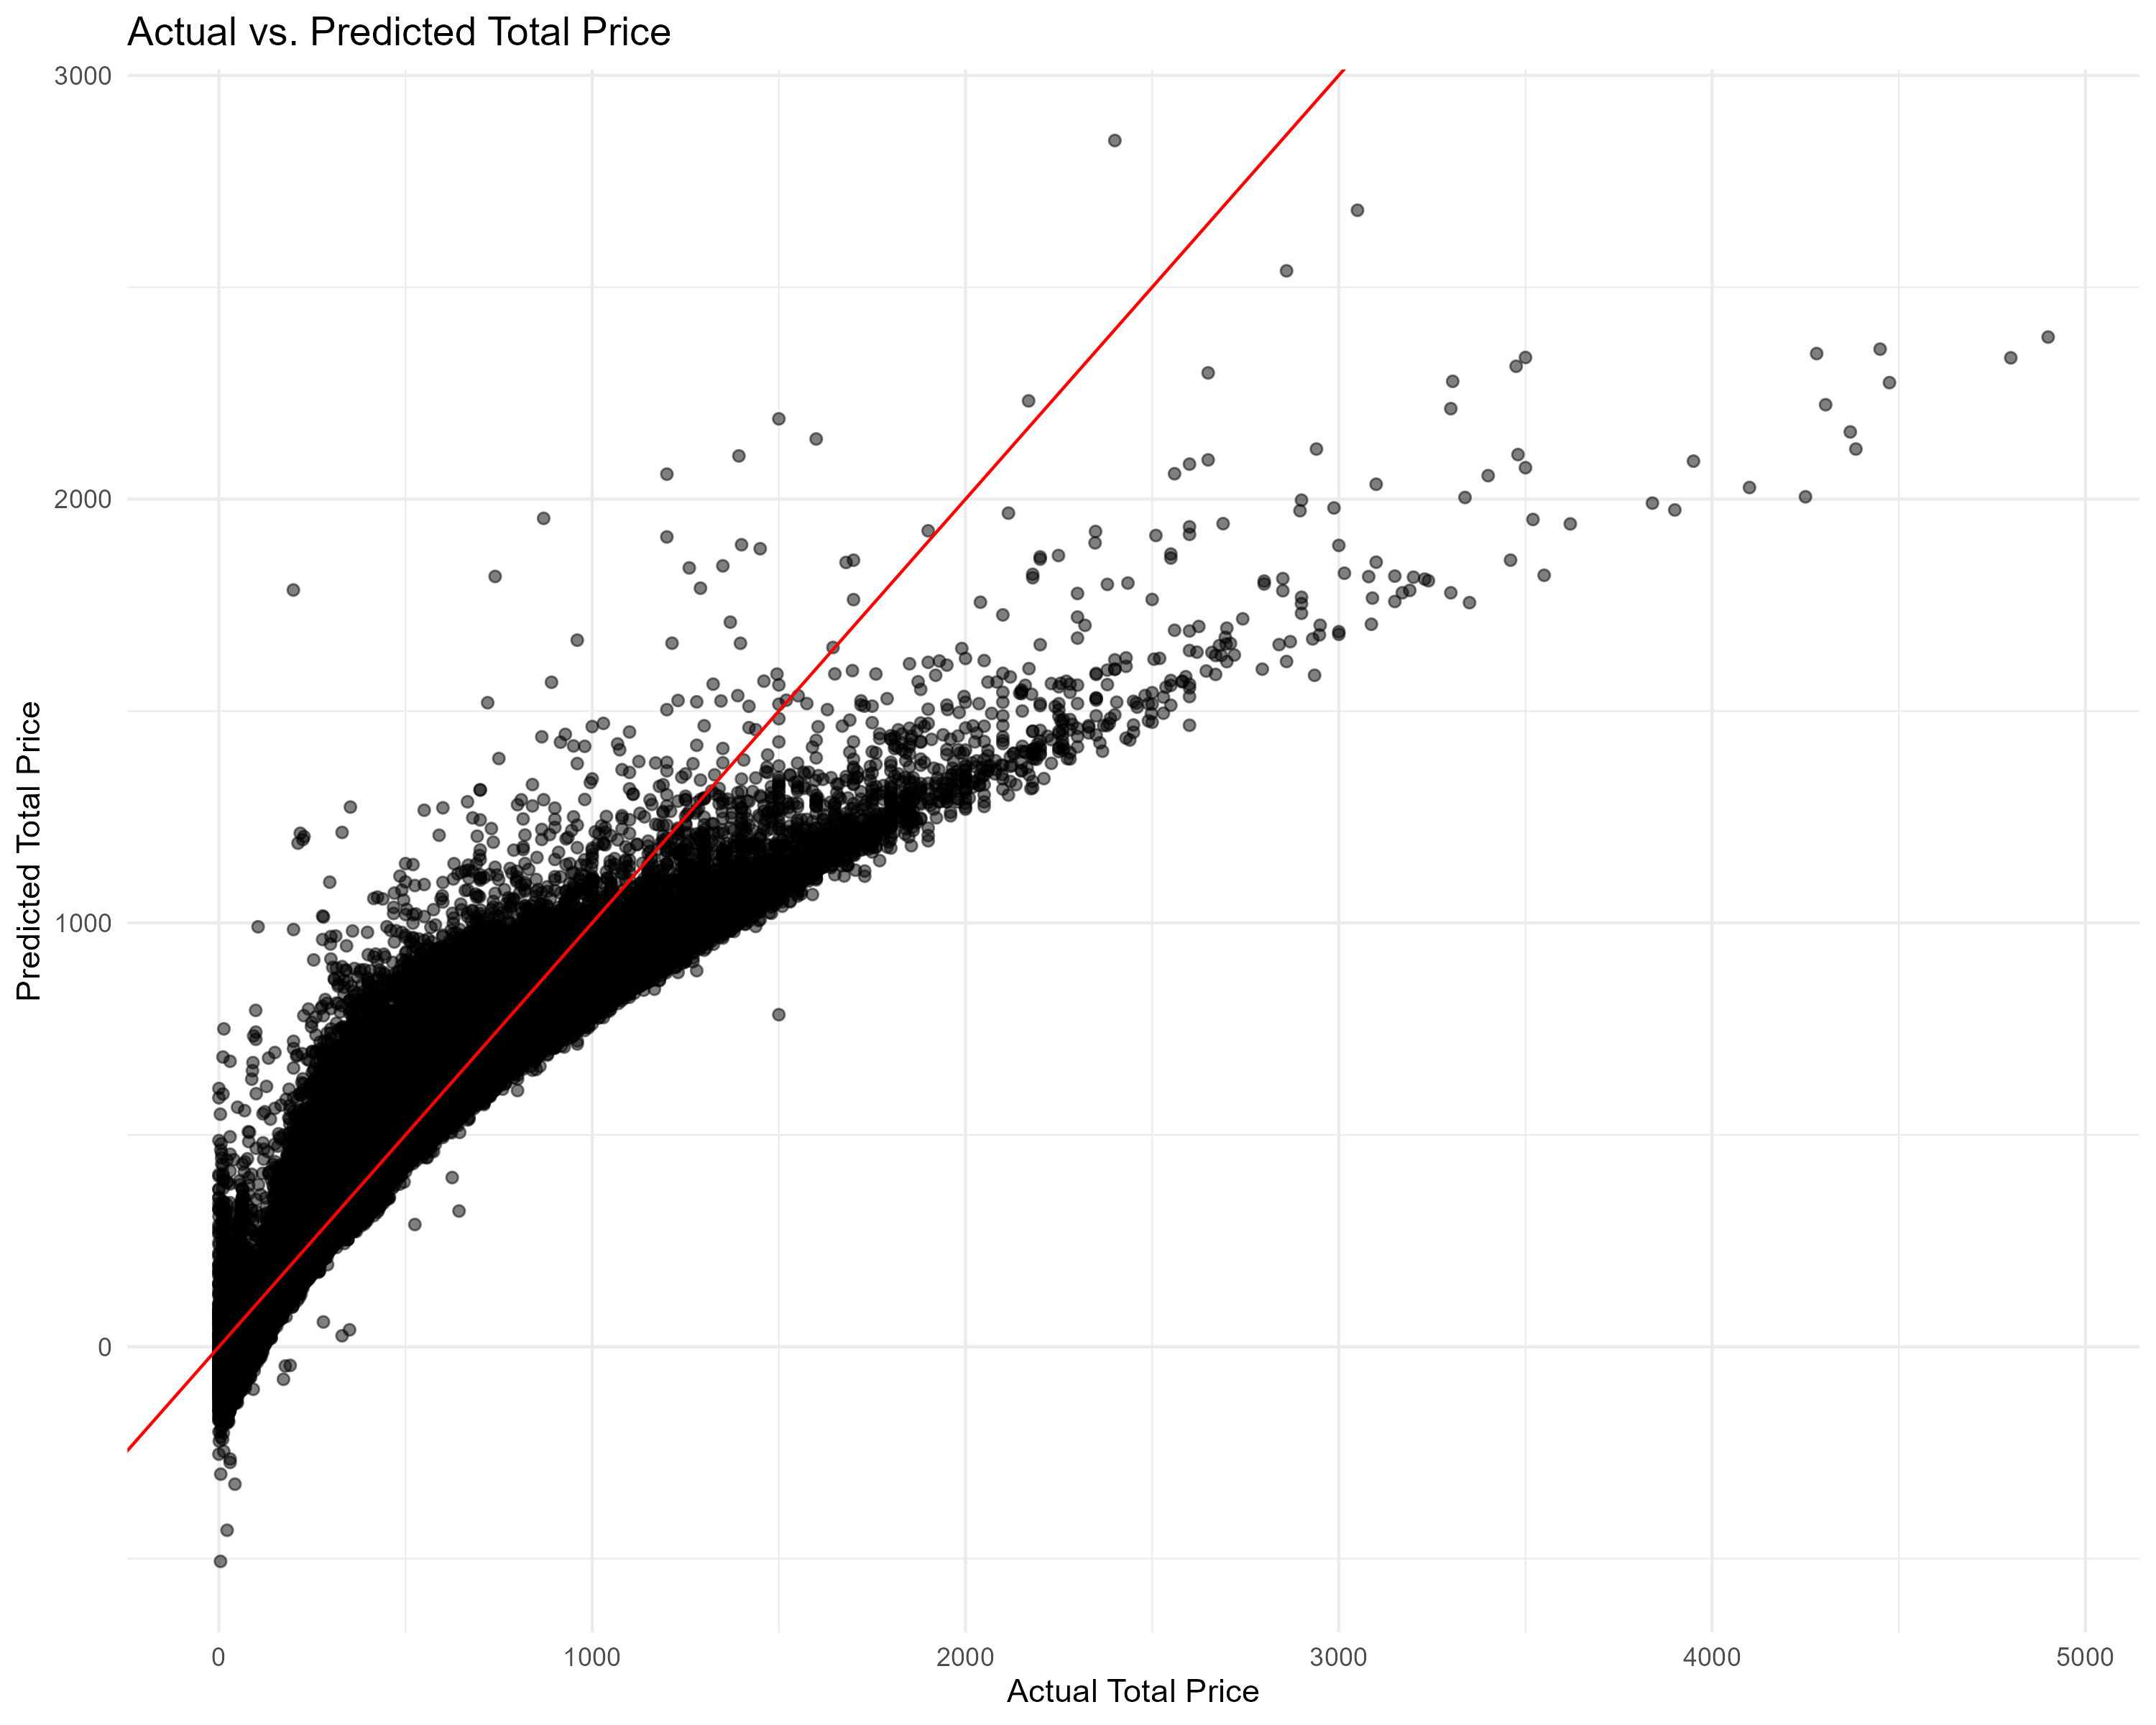
\includegraphics{../results/price_prediction_plot.png}

}

\caption{\label{fig-prediction-model}Prediction Model}

\end{figure}%

Table~\ref{tbl-model} is the statistical summary of our linear
regression model, which is built to predict house prices in Beijing,
with the response variable totalPrice and various explanatory variables.
The model excludes constructionTime and buildingType from the analysis.

The model has a high Multiple R-squared value of 0.8831, indicating a
strong fit to the data.

Figure~\ref{fig-prediction-model} compares actual price and predicted
total prices from the model, with a red line representing perfect
prediction. Points close to this line are predictions that match closely
with actual prices, whereas points further away represent less accurate
predictions. Figure~\ref{fig-prediction-model} shows a strong positive
correlation, but with a certain degree of variance as prices increase,
suggesting that while the model predicts lower-priced houses quite
accurately, it is less precise with higher-priced ones.

The present study employed a linear regression model to conduct an
in-depth analysis of the key determinants of housing prices in the
Beijing real estate market. The model exhibits a strong overall fit,
with an R-squared of 0.8821, indicating that it is able to explain
approximately 88.21\% of the variation in housing prices. The
F-statistic of 65,750 with a p-value less than 2.2e-16 suggests that the
model is highly statistically significant. Examining the coefficient
estimates, several key findings emerge. First, locational factors play a
significant role in shaping housing prices. The model indicates that
prices tend to decrease as the longitude (i.e., eastward location)
increases and increase as the latitude (i.e., northward location) rises.

Second, the time-related variables show interesting patterns. The number
of days the property has been on the market (trade time) has a positive
and highly significant association with prices, suggesting that
properties that have been listed for longer tend to command higher
prices, all else equal. The number of followers a property has is also
positively related to prices, though the effect size is relatively
small.

Regarding the physical property characteristics, the results are
consistent with standard hedonic pricing theory. Larger living area,
more kitchens, and more bathrooms are associated with higher prices.
Interestingly, the number of living rooms and drawing rooms have
negative impacts on prices, potentially indicating a preference for more
functional living spaces in this market.

The building structure and renovation condition also matter. Properties
with brick/wood construction tend to have lower prices compared to other
building types, while homes with steel/concrete structures command
higher prices. The condition of renovations also plays a role, with
rough and simplistic renovations associated with lower prices relative
to more extensive renovations. In terms of accessibility and ownership
factors, the model reveals that properties without elevators have higher
prices, potentially due to lower construction costs. Homes not located
near a subway station also tend to have higher prices. However, the
length of property ownership does not appear to have a significant
effect on prices.

Lastly, the model identifies substantial spatial variation in housing
prices across different districts in Beijing. Several districts, such as
Chaoyang, Daxing, Fangshan, and Tongzhou, have significantly higher
prices compared to the baseline, while the Xicheng district has lower
prices. Additionally, the average price in the surrounding community is
a strong positive predictor of individual property prices, highlighting
the importance of local market conditions and amenities. Overall, this
comprehensive regression analysis provides rich statistical evidence to
deepen the understanding of the price formation mechanisms in the
Beijing real estate market. While the linear framework has achieved good
explanatory power, there may still be some heterogeneity and non-linear
effects that warrant further exploration. Future research could
experiment with more complex modeling approaches to further enhance the
predictive accuracy and provide more precise insights to inform relevant
decision-making.

\subsection*{references}\label{references}
\addcontentsline{toc}{subsection}{references}

\phantomsection\label{refs}
\begin{CSLReferences}{1}{0}
\bibitem[\citeproctext]{ref-han2021winning}
Han, X., Y. Shen, and B. Zhao. 2021. {``Winning at the Starting Line:
The Primary School Premium and Housing Prices in Beijing.''} \emph{China
Economic Quarterly International} 1 (1): 29--42.
\url{https://doi.org/10.1016/j.ceqi.2020.12.001}.

\bibitem[\citeproctext]{ref-hou2010housing}
Hou, Y. 2010. {``Housing Price Bubbles in Beijing and Shanghai?: A
Multi‐indicator Analysis.''} \emph{International Journal of Housing
Markets and Analysis} 3 (1): 17--37.
\url{https://doi.org/10.1108/17538271011027050}.

\bibitem[\citeproctext]{ref-qin_han_2013}
Qin, Bo, and Sun Sheng Han. 2013. {``Emerging Polycentricity in Beijing:
Evidence from Housing Price Variations, 2001--05.''} \emph{Urban
Studies} 50 (10): 2006--23.
\url{https://doi.org/10.1177/0042098012471979}.

\bibitem[\citeproctext]{ref-ZHANG201872}
Zhang, Lei, and Yimin Yi. 2018. {``What Contributes to the Rising House
Prices in Beijing? A Decomposition Approach.''} \emph{Journal of Housing
Economics} 41: 72--84.
https://doi.org/\url{https://doi.org/10.1016/j.jhe.2018.04.003}.

\end{CSLReferences}



\end{document}
